\documentclass[a4paper]{report}

\usepackage{../mathstemplate}

\date{IV семестр, весна 2024 г.}
\title{Дифференциальная геометрия. Неофициальный конспект}
\author{Лектор: Нина Дмитриевна Лебедева \\ Конспектировал Леонид Данилевич \\ Редактировал Максим Лаунер}

\begin{document}
    \shorthandoff{"}
    \maketitle
    \tableofcontents
    \newpage
    \setcounter{lection}{0}


    \chapter{Основные понятия}
    \newlection{14 февраля 2024 г.}
    \section{Гладкие многообразия}
    \definition[Топологическое многообразие]{
        Хаусдорфово топологическое пространство $M$ со счётной базой, такое что $\forall x \in M: \exists U \ni x: U \sim \R^n$.
        Данное число $n$ называется \emph{размерностью} многообразия, пишут $\dim M = n$, или же часто пишут это число верхним индексом: $M^n$.
    }
    Далее пусть $M^n$ --- топологическое многообразие.
    \definition[Карта]{
        Пара из открытого $U \subset M^n$, и гомеоморфизма $\phi: U \map \Omega$, где открытое $\Omega \subset \R^n$.
    $U$ называется \emph{носителем карты}.
    }
    <<В половине случаев в литературе картой называется обратное отображение>>.
    \definition[Атлас]{
    Набор карт $(U_i, \phi_i)$, таких, что $\bigcup\limits_{i}U_i = M$.
    }
    Пусть даны две карты $(U, \phi)$ и $(V, \psi)$.
    Далее удобно считать, что их носители пересекаются: $U \cap V \ne \o$, иначе определение не несёт смысла.
    \definition[Отображение перехода]{
    Отображение $\psi \circ \phi^{-1}: \phi(U \cap V) \map \psi(U \cap V)$. Обозначается $f_{\phi\psi}$.
    }
    \definition[Карты $(U, \phi)$ и $(V, \psi)$ согласованы]{
        Отображение перехода и ему обратное гладкие.
    }
    \definition[Гладкий атлас]{
    Атлас, такой, что любые две карты согласованы.
    }
    Далее все атласы предполагаются гладкими.
    \definition[Атласы эквивалентны]{
        Их объединение (то есть все карты из первого и из второго атласа вместе взятые) --- тоже гладкий атлас.
    }
    \proposal{
    Эквивалентность атласов --- отношение эквивалентности.
    }
    \definition[Гладкая структура на многообразии]{
    Максимальный гладкий атлас (атлас, к которому нельзя добавить карт).
    }
    \note{
        К атласу можно добавить произвольное количество карт, согласованных с теми, что в атласе, и они будут согласованы между собой.
    В частности, для задания гладкой структуры достаточно произвольного атласа $A$: в $A$ можно добавить всевозможные карты, согласованные с картами из $A$, и он станет максимальным.
    }
    \definition[Гладкое многообразие]{
    Многообразие с гладкой структурой.
    }
    \examples[Атласы]{
    \item Стандартная гладкая структура на $\R^n$ задаётся атласом $\{(\R^n, \id)\}$.
        \item В частности, стандартная структура на $\R^1$ задаётся атласом $\{(\R^1, [x \mapsto x])\}$.
    \item Можно задать нестандартную структуру на $\R^1$: $\{(\R^1, [x \mapsto x^3])\}$.
    \precaution{
        Это действительно гладкая структура, хотя обратное отображение ${[x \mapsto x^{\nicefrac{1}{3}}]}$ не гладкое.
        Тем не менее, определение и не требует гладкости от него.
    }
    \item Пусть $f = \all{x, & x \ge 0 \\ \frac{1}{2}x,&x \le 0}$. Тогда $\{(\R^1, f)\}$ --- тоже гладкий атлас на $\R^1$.

    Тем не менее, любые два атласа из приведённых выше атласов на $\R^1$ не эквивалентны --- отображения перехода получаются не гладкими.
    \item Гладкая структура на сфере задаётся двумя картами: пусть $S^2$ --- сфера с северным полюсом $N$ и южным $S$, пусть $f, g$ --- стереографические проекции с данными полюсами.
        Тогда ${\{(S^2 \sm \{N\}, f), (S^2 \sm \{S\}, g)\}}$ --- атлас.
    }
    \note{
    Если $M$ --- гладкое многообразие, и открытое $W \subset M$, то на $W$ естественным образом определена гладкая структура, наследующаяся с $M$.
    }
    \subsection{Гладкие отображения}

    Пусть $M^m, N^n$ --- гладкие многообразия, $A_M, A_N$ --- соответствующие атласы.
    Рассмотрим отображение $f: M \map N$.
    \definition[Координатное представление $f$ в картах $(U, \phi)$ на $M$ и $(V, \psi)$ на $N$]{
        Такое $\tilde{f}: \phi(U) \map \psi(V)$, что диаграмма коммутативна везде, где определена (то есть $\tilde{f} = \psi \circ f \circ \phi^{-1}$ на $\phi(U \cap f^{-1}(V))$).
        % https://q.uiver.app/#q=WzAsNCxbMCwxLCJcXHBoaShVKSJdLFsxLDEsIlxccHNpKFYpIl0sWzAsMCwiVSJdLFsxLDAsIlYiXSxbMiwwLCJcXHBoaSJdLFszLDEsIlxccHNpIl0sWzIsMywiZiJdLFswLDEsIlxcdGlsZGV7Zn0iXV0=
        \[\begin{tikzcd}[ampersand replacement=\&]
              U \& V \\
              {\phi(U)} \& {\psi(V)}
              \arrow["\phi", from=1-1, to=2-1]
              \arrow["\psi", from=1-2, to=2-2]
              \arrow["f", from=1-1, to=1-2]
              \arrow["{\tilde{f}}", from=2-1, to=2-2]
        \end{tikzcd}\]
    }
    Далее считаем, что $f: M \map N$ непрерывна (эквивалентно, все координатные представления непрерывны).
    \definition[$f$ гладкое]{
    Любое координатное представление --- гладкое.
    }
    \definition[$f$ --- гладкое в точке $x \in M$]{
    Найдётся окрестность $U_x \ni x$ и карты $(U, \phi)$, $(V, \psi)$ (где $V \ni y \coloneqq f(x)$), такие, что $U_x \subset U$ и сужение на $U_x$ координатного представления $f$ --- гладко.
    }
    \properties[Гладкие отображения]{
    \item Гладкость в точке не зависит от выбора карт.
    \item Гладкость отображения не зависит от выбора атласа в одном классе эквивалентности.
    \item Отображение гладкое $\iff$ оно гладкое в любой точке. \comment{На лекции было доказательство $\when$.}
    \item Пусть $f: M \map N, g: N \map K$ гладкие. Тогда их композиция $g \circ f$ гладкая.
    \item Тождественное отображение гладкое, если в образе и прообразе выбраны эквивалентные атласы.
    \item Определение гладкости отображения совпадает с определением гладкости из матанализа (если считать, что $M \subset \R^m, N \subset \R^n$ открыты, и порождающие атласы наследуют структуры $\R^m$ и $\R^n$)
    }
    \definition[Диффеоморфизм $f: M \map N$]{
    Гладкое $f$, такое, что $f^{-1}$ --- тоже гладкое.
    }
    \definition[Многообразия $M$ и $N$ диффеоморфны]{
    Между ними существует диффеоморфизм.
    }
    Понятно, что диффеоморфность --- отношение эквивалентности.
    \statement{
    Если $M^m \overset{\text{диф}}\sim N^n$, то $m = n$.
    \provehere{
    Рассмотрим произвольную $x \in M$.
    Пусть $f: M \map N$ --- диффеоморфизм, пусть $\tilde{f}$ --- его координатное представление.
        Тогда $\tilde{f}^{-1}$ --- координатное представление $f^{-1}$, откуда $\tilde{f}^{-1}$ --- тоже гладкое.
     Рассмотрим дифференциал $\d_x{\tilde{f}}(\_)$, это изоморфизм векторных пространств, значит, $m = n$.
    }
    }
    По умолчанию всегда считается, что на $\R^m$ введена стандартная гладкая структура.
    \proposal{
        Пусть $M$ --- гладкое многообразие, тогда карта --- диффеоморфизм между $U$ и $\phi(U)$.
        Обратно, любой диффеоморфизм между открытым подмножеством $W \subset M$ и областью $\Omega \subset \R^m$ --- карта.
        \provehere{
        \[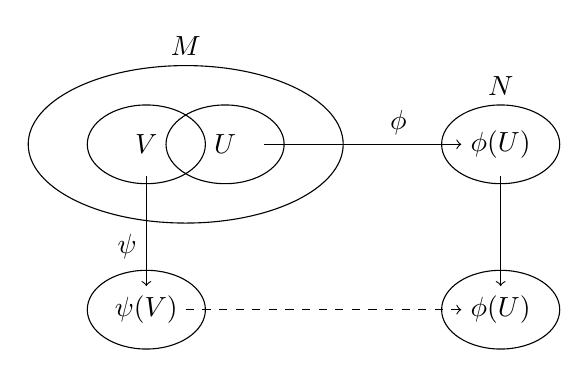
\begin{tikzpicture}
              \draw (-2,2) ellipse (2cm and 1cm);
              \draw (-2.5,2) ellipse (0.75cm and 0.5cm);
              \draw (-1.5,2) ellipse (0.75cm and 0.5cm);
              \node at (-2.5,2) {$V$};
              \node at (-1.5,2) {$U$};
              \node[above] at (-2,3) {$M$};
              \draw[->] (-1, 2) -- (1.5,2);
              \node[above] at (0.7,2) {$\phi$};
              \draw (2,2) ellipse (0.75cm and 0.5cm);
              \node at (2,2) {$\phi(U)$};
              \node[above] at (2,2.5) {$N$};
              \draw[->] (2,1.6) -- (2,0.2);
              \node[right] at (2,1) {$\id$};
              \draw (2,-0.1) ellipse (0.75 cm and 0.5 cm) node {$\phi(U)$};
              \draw[->] (-2.5,1.6) -- (-2.5,0.2);
              \node[left] at (-2.5, 0.7) {$\psi$};
              \draw (-2.5,-0.1) ellipse (0.75 cm and 0.5 cm) node {$\psi(V)$};
              \draw[->,dashed] (-2,-0.1) -- (1.5,-0.1);
        \end{tikzpicture}\]
            Гладкость карты, как диффеоморфизма, эквивалентна тому, что карта согласована с остальными в атласе: пунктирная стрелка $\psi(U \cap V) \map \phi(U \cap V)$ одновременно является и отображением перехода между картами $(U, \phi)$ и $(V, \psi)$, и координатным представлением $\phi$ в картах $(V, \psi), (U, \id)$.
        }
    }
    \corollary{Диффеоморфизм $f: M \map N$ задаёт естественную биекцию между картами $M$ и картами $N$ (а ещё между (максимальными) атласами $M$ и (максимальными) атласами $N$). }
    \newlection{21 февраля 2024 г.}
    \example[Диффеоморфизм]{
        Ранее приводились неэквивалентные карты $(\R, \id)$ и $(\R, [x \mapsto x^3])$.
        Вещественные прямые с данными картами диффеоморфны: $[x\mapsto x^3]$ --- диффеоморфизм, ему обратный $\left[x \mapsto \sqrt[3]{x}\right]$ $\left(\textrm{где, как в школе, }\sqrt[3]{x} = \all{\sqrt[3]{x},&x \ge 0 \\ -\sqrt[3]{-x},&x < 0}\right)$.
    }
    Таким образом, создать две недиффеоморфные структуры на одном и том же многообразии не то чтобы просто.
    \intfact{
    Пусть $M$ --- $n$-мерное многообразие.

        Если $\all{n < 4,&\text{на нём существует единственная гладкая структура} \\ n = 4,&\text{на нём существует бесконечно много гладких структур} \\ n>4,&\text{на нём существует конечное число гладких структур}}$.

        В частности, при $n > 4$: если $M^n = \R^n$, то гладкая структура единственна.
    }
    \subsection{Касательное пространство}
    Пусть $M$ --- гладкое многообразие, $p \in M$.
    Пусть $\alpha, \beta: (-\eps, +\eps) \map M$ --- гладкие (естественно, в смысле отображения многообразий) кривые, такие, что $\alpha(0) = p = \beta(0)$.
    \definition[$\alpha$ и $\beta$ соприкасаются в $p$]{
        В любой карте $(U, \phi)$ (где $U \ni p$) их производные в нуле совпадают: $(\phi \circ \alpha)'(0) = (\phi \circ \beta)'(0)$.
    }
    \precaution{
    Определение требует совпадение векторов скорости, а не просто параллельности или сонаправленности.
    }
    \properties[Соприкасающиеся кривые]{
    \item Соприкасаемость кривых в какой-то конкретной точке --- отношение эквивалентности.
    \item Соприкасаемость не зависит от выбора карты: достаточно проверить в любой одной, содержащей $p$.
    \provehere{
        Пусть $(U, \phi)$, $(V, \psi)$ --- две карты, содержащие точку $p$, отображение $f_{\phi\psi} = \psi\circ\phi^{-1}$ гладкое, значит, его дифференциал переводит равные векторы в равные.
    }
    }
    \definition[Касательный вектор в точке $p \in M$]{
    Класс эквивалентности соприкасающихся в точке $p$ кривых.
    }
    Множество всех касательных векторов --- \emph{касательное пространство}, обозначают $T_p M$.
    \subsubsection{Координаты касательного вектора}
    Пусть $p \in M$, и $(U, \phi)$ --- карта, содержащая $p$.
    \definition[Координатное представление вектора $v = \lbrack\alpha\rbrack \in T_p M$]{
        Вектор скорости данной кривой в данной карте $v_\phi \bydef (\phi \circ \alpha)'(0)$.
    }
    Понятно, что определение не зависит от выбора представителя --- кривой $\alpha$.

    Также координаты $v_\phi$ в $\R^n$ называют \emph{координатами $v$ в карте $\phi$}.
    \properties[Координатное представление]{
    \item $\forall p \in M, \forall (U, \phi): p \in U \then$ координатное представление --- биекция $T_p M \map \R^n, v \mapsto v_\phi$.
    \provehere{
    Это инъекция, так как если образы $u, v$ равны, то по определению $u$ и $v$ соприкасаются.

        Это сюръекция: $\forall w \in \R^n$ можно рассмотреть кривую $\gamma: \R \map \R^n, \gamma(t) \coloneqq w t + \phi(p)$.
        Координаты $[\phi^{-1} \circ \gamma]$ в карте $\phi$ как раз окажутся равными $w$.
    }
    }
    \subsubsection{Преобразование координатного представления в зависимости от карты}
    \statement{\label{change-map}
        Пусть $M^n \ni p$ --- гладкое многообразие и точка, $(U, \phi)$ и $(V, \psi)$ --- карты, содержащие $p$. Тогда $v_\psi = \d_{\phi(p)}{f_{\phi\psi}}(v_\phi)$.
        \provehere{
            Пусть $v = [\alpha]$. Тогда $v_\phi = (\phi \circ \alpha)'(0)$, $v_\psi = (\psi \circ \alpha)'(0)$, и действительно, так как $f_{\phi\psi} = \psi\circ\phi^{-1}$, то $v_\psi = (f_{\phi\psi} \circ \phi \circ \alpha)'(0)$.
            Дифференцируя композицию, получаем утверждение.
        }
    }
    Следствием данного утверждения является альтернативное определение касательного вектора:
    \definition[Касательный вектор в точке $p \in M$]{
    Отображение из множества всех карт, содержащих точку $p$ (обозначим их $\mathcal{M}_p$) в $\R^n$
    \[\mathcal{M}_p \map \R^n\]
    такое, что выполнены соотношения~(\cref{change-map}).
    }
    Можно показать, что данное определение, и определение через соприкасающиеся кривые, эквивалентны.

    Это определение сродни тому определению тензора, которое говорит: <<Тензор --- это многомерная матрица чисел, преобразующихся при замене базиса следующим образом\dots>>
    \subsection{Структура векторного пространства на $T_p M$}
    Зафиксируем $p \in M$, и карту $(U, \phi)$, содержащую $p$.
    Пусть $v, w \in T_p M$.
    \definition[Сумма векторов $v$ и $w$]{ Такой вектор $v + w$, что $(v + w)_\phi = v_\phi + w_\phi$.}
    \definition[Растяжение вектора $v$ с коэффициентом $\alpha$]{ Такой вектор $\alpha v$, что $(\alpha v)_\phi = \alpha \cdot v_\phi$.}
    Иными словами, у нас была биекция $T_p M$ с векторным пространством, и мы просто перенесли структуру векторного пространства с $\R^n$ на $T_p M$.
    Определение не зависит от выбора карты, так как замена координат касательных векторов при переходе между картами --- изоморфизм векторных пространств (дифференциал --- линейный оператор).
    \note{
        Из определения получается, что $v \map v_\phi$ --- изоморфизм векторных пространств.
    }
    \section{Касательное расслоение}
    Как множество, $T(M) = \bigsqcup\limits_{p \in M}T_p M$.
    Оказывается, на $T(M)$ можно естественно ввести топологию и гладкую структуру размерности $2n$.
    Преобразуем определение атласа так, чтобы это случилось одновременно.

    \statement[Атлас для множества]{
        Пусть $X$ --- множество с картами $(U, \phi)$, то есть парами $(U, \phi)$ где $U \subset X$, и каждая $\phi$ --- биекция $U \map \R^n$. При этом $X = \bigcup U$

        Потребуем для любых двух карт $(U, \phi)$ и $(V, \psi)$: $\phi(U \cap V)$ открыто (в частности, $\phi(U)$ открыто), и потребуем, чтобы все функции перехода $f_{\phi\psi} = \psi \circ \phi^{-1}$ были гладкими.

        Введём на $X$ топологию: $W \subset X$ открыто, если $\forall (U, \phi): \phi(U \cap W)$ открыто, и предположим, что топология получилась хаусдорфовой, и что на $X$ есть счётная база.

        Тогда утверждается, что данная процедура задаёт на $X$ одновременно и топологию, и гладкую структуру.
    }
    Зададим такую гладкую структуру на $T(M)$.
    Обозначим $T U = \bigsqcup\limits_{p \in U}T_p M$.
    Можно рассматривать $TU$ как множество пар, состоящих из точки и вектора: $TU = \defset{(p, v)}{p \in U, v \in T_p M}$.

    Пусть имеется карта $(U, \phi)$ на $M$.
    Построим по ней карту \begin{align*}\Phi: TU &\map \R^n \times \R^n \\ (p, v) & \mapsto (\phi(p), v_\phi)\end{align*}

    Проверим согласованность: пусть $(U, \phi)$ и $(V, \psi)$ --- две карты на $M$.
    По ним построены карты $(TU, \Phi)$ и $(TV, \Psi)$ соответственно.
    Тогда $(\Psi \circ \Phi^{-1})(p, v) = ((\psi \circ \phi^{-1})(p), \d_{\phi(p)}{f_{\phi\psi}}(v))$, видно, что $\Psi \circ \Phi^{-1}$ гладко.

    \exercise{
    Получилось хаусдорфовое пространство со счётной базой.
    }
%    \comment{На лекции леммы ниже не было, но давайте для порядка докажем. Проверка свойств всё равно остаётся читателю в качестве упражнения.}
%    \lemma{
%        Получилось хаусдорфово пространство со счётной базой.
%        \provebullets{
%        \item Проверим хаусдорфовость. Рассмотрим две точки $(p_1, v_1), (p_2, v_2) \in TM$.
%
%            Пусть $p_1 \ne p_2$. Выберем карты $(U_1, \phi_1)$ и $(U_2, \phi_2)$, где $p_i \in U_i$.
%            Так как $M$ хаусдорфово, а атлас максимальный, то можно считать, что $U_1 \cap U_2 = \o$ (при необходимости уменьшить $U_1$ и $U_2$).
%            Множества $T U_1$ и $T U_2$ открыты в $TM$ и являются непересекающимися окрестностями $p_1$ и $p_2$.
%
%            Теперь пусть $p_1 = p_2$, $v_1 \ne v_2$. Выберем карту $(U, \phi)$, где $p \in U$, по ней построена карта $(TU, \Phi)$.
%            Из хаусдорфовости $\R^n$ найдётся непересекающиеся окрестности $v_1$ и $v_2$, пусть это $V_1$ и $V_2$ соответственно.
%
%            Тогда $\Phi^{-1}(V_1)$ и $\Phi^{-2}(V_2)$ --- непересекающиеся окрестности $(p_1, v_1)$ и $(p_2, v_2)$.
%        \item Пусть на $M$ имеется счётная база $\{U_i\}_{i \in I}$, возьмём в $\R^n$ какую-то счётную базу $\{V_j\}_{j \in J}$.
%
%            Пусть $\mathcal{U} \coloneqq \defset{U_i}{i \in I, \exists \phi_i: (U_i, \phi_i)\text{ --- карта}}$.
%            В следующем абзаце покажем, что $\mathcal{U}$ --- тоже (понятно, счётная) база.
%
%            Рассмотрим произвольное открытое $U \subset M$, и $p \in U$. Пусть имеется карта $\left(\tilde{U}, \tilde{\phi}\right)$, содержащая $p$, тогда $U \cap \tilde{U}$ открыто, и по критерию базы имеется $U_i$ ($i \in I$), такое, что $p \in U_i \subset U \cap \tilde{U}$.
%            Так как атлас максимален, то $\left(U_i, \tilde{\phi}\big|_{U_i}\right)$ --- карта.
%
%            Раз $\mathcal{U}$ --- счётная база, то считаем, что эта база совпадает с $\{U_i\}_{i \in I}$.
%            Пусть по карте $(U_i, \phi_i)$ построена карта $(T U_i,\Phi_i)$, тогда $\{\Phi_i^{-1}(\phi_i(V_j))\}_{i \in I, j \in J}$ --- счётная база в $TM$.
%        }
%    }
    \subsection{Дифференциал гладкого отображения}
    Пусть $M$ и $N$ --- гладкие многообразия, и есть гладкое отображение $f: M \map N$.
    Зафиксируем $p \in M$.
    \definition[Дифференциал $f$ в точке $p$]{
    Отображение $\d_p f: T_p M \map T_{f(p)}N$, заданное следующим образом: $\d_p f: [\alpha] \mapsto [f \circ \alpha]$.
    }
    \statement{
        Определение дифференциала не зависит от выбора представителей.
        \provehere{
            Пусть $\alpha \sim \beta$ --- две кривые, $\alpha(0) = \beta(0) = p$, $\alpha'(0) = \beta'(0) = v$.

            Проверим, что $f \circ \alpha \sim f \circ \beta$.
            Достаточно проверить, что совпадают координатные представления.

            Выберем две карты $(U, \phi)$ и $(V, \psi)$ (где $U \ni p$, $V \ni f(p)$).
            Координатное представление $f$ --- это $\tilde{f} = \psi \circ f \circ \phi^{-1}$.

            Дифференциал $\tilde{f}$ переносит координаты представления векторов из $T_p M$ в координаты представления векторов из $T_{f(p)}N$:
        \gather{\psi \circ f \circ \alpha = \tilde{f} \circ \phi \circ \alpha \text{\quadи\quad}\psi \circ f \circ \beta = \tilde{f} \circ \phi \circ \beta\\ (\psi \circ (f \circ \alpha))'(0) = \d_{\phi(p)} \tilde{f}((\phi \circ \alpha)'(0)) = \d_{\phi(p)} \tilde{f}((\phi \circ \beta)'(0)) = (\psi \circ (f \circ \beta))'(0)\qedhere }
        }
    Нетрудно заметить, что $(\d_p f(v))_\psi = \left(\d_{f(p)}\tilde{f}\,\right)(v_\phi)$ в обозначениях из доказательства выше (и $v = [\alpha]$).
    \corollary{
        $\d_p f$ --- линейное отображение.
    }
    }
    \newlection{28 февраля 2024 г.}
    \note{
    Можно естественным определить дифференциал на всём пространстве $TM$ вот так: $T f: T M \map T N$.
        На вектор $v \in T_p M$ отображение $T f$ действует понятным образом: $v \mapsto \d_p f(v)$.
    }
    Если $U \subset \R^n$, то касательное пространство $TU$ естественным образом отождествляется с $U \times \R^n$.
    \section{Гладкие векторные поля}
    Пусть $M$ --- гладкое многообразие, выберем произвольное подмножество $A \subset M$.

    \definition[Непрерывное векторное поле на $A$]{
        Непрерывное отображение $X: A \map TM$, такое, что $\forall p \in A: X(p) \in T_p M$.
        Часто пишут $X_p$ вместо $X(p)$.
    }

    \definition[Гладкое векторное поле на $A$]{
        Векторное поле $X: A \map TM$, такое, что $\exists$ открытое $U \subset M: U \supset A$, и $X$ продолжается на $U$, как гладкое векторное поле (то есть гладкое отображение $U \map TM$, являющееся непрерывным векторным полем).
    }
    Для гладкого многообразия $M$ будем обозначать пространство всех гладких векторных полей за $\mathscr{X}(M)$.

    Пусть в $M$ имеется карта $(U, \phi)$.
    Векторные поля задавались на подмножестве $A \subset M$, а не на всём многообразии, так как один из самых частых примеров гладкого векторного поля --- \emph{координатное векторное поле} --- задаётся лишь в карте $U$:
    \definition[Координатное векторное поле, соответствующее $i$-й координате]{
        Векторное поле $V_i: U \map TM$, такое, что $\d \phi(V_i) = e_i$ (с координатами $V_i(p)_{\phi} = e_i$).
    }
    \lemma{
        Пусть имеется открытое $U \subset \R^n$, и компактное $K \subset U$.
    Утверждается, что $\forall V \supset K: \Cl V \subset U \then$ можно построить гладкую функцию $f: \R^n \map \R$, такую, что $f\big|_{K} = 1$, $f\big|_{\R^n \sm V} = 0$.
    \provehere{
    $\R^n \sm V$ замкнуто, значит, $d \coloneqq \dist(\R^n \sm V, K) > 0$.
        Функция $\chi_{K}$ почти подходит, только она не гладкая.
        Немножко увеличим носитель: рассмотрим $W \coloneqq U_{\nicefrac{d}{2}}(K) = \defset{x \in \R^n}{\dist(x, K) < \frac{d}{2}}$.
        Для $\chi_{W}$ условие выполняется и в окрестности $K$, а, значит, подойдёт свёртка $\chi_{W} \circ g_{\frac{d}{2}}$, где $g_{\frac{d}{2}}$ --- подходящая аппроксимативная единица, гладкая функция с компактным носителем, равная нулю вне $B_{\frac{d}{2}}(0)$.
    }
    }
    \corollary{\label{extension-of-coordinates}
        Пусть $V_i$ --- координатное поле карты $(U, \phi)$.
        Тогда $\forall K \subset U: \exists$ векторное поле $\tilde{V}_i: \tilde{V}_i\big|_{K} = V_i, \tilde{V}_i\big|_{M \sm U} \equiv 0$.

    Иными словами, всегда немного уменьшив карту, можно продолжить координатное векторное поле на всё многообразие.
    }
    \section{Гладкие подмногообразия}
    Пусть $M^m$ --- гладкое многообразие размерности $m$.
    \definition[Гладкое подмногообразие размерности $n \le m$]{
    Подмножество $N \subset M$, такое, что $\forall p \in N: \exists$ выпрямляющая карта $(U, \phi)$ (карта на $M$), такая, что $U \ni p$ и $\phi(U) \cap \R^n = \phi(N \cap U)$.
    }
    Здесь имеется в виду, что $\phi$ действует в $\R^m$, и имеется определённое вложение $\R^n \hookrightarrow \R^m$ (скажем, в $\R^m$ выбран базис, и на первые $n$ векторов натянуто $\R^n$).
    \statement{
    На $N$ каноническим образом индуцируется гладкая структура из $M$. Карты на $N$ --- сужения выпрямляющих карт (карте $(U, \phi)$ отвечает карта $(N \cap U, \psi)$, где $\psi: N \cap U \map \R^n \subset \R^m$, $\psi(x) = \phi(x)$).
    \provehere{
    Согласованность карт на $N$ следует из согласованности карт на $M$.
    }
    }
    Пусть $N^n, M^m$ --- гладкие многообразия.
    \definition[Погружение $f: N \map M$]{
    Гладкое отображение $f: N \map M$, такое, что $\forall p \in N: \d_p f$ --- инъекция.
    Само $f$ не обязано быть инъекцией.
    }
    Понятно, что такое возможно только при $n \le m$.
    \definition[Вложение $f: N \map M$]{
        Погружение $f: N \map M$, которое является топологическим вложением, то есть гомеоморфизмом на образ.
    }
    \examples{
    \item В случае поверхностей размерности $2$ погружение подмногообразия размерности $1$ --- кривой --- называлось регулярной параметризацией.
    \item Петля слева является погружением, но даже инъективная петля справа вложением не является: в выделенной точке топология не совпадает с топологией интервала.
        \[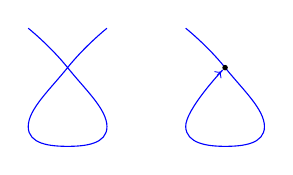
\begin{tikzpicture}
              \draw[blue] plot [smooth,tension=0.8] coordinates {(-0.5,0.5) (0,0) (0.5,-0.75) (0,-1) (-0.5,-0.75) (0,0) (0.5,0.5)};
              \draw[blue] plot [smooth,tension=0.8] coordinates {(1.5,0.5) (2,0) (2.5,-0.75) (2,-1) (1.5,-0.75) (1.97,-0.03)};
              \draw[blue,->] (1.9,-0.1) -- (1.95,-0.05);
              \fill (2,0) circle (1pt);
        \end{tikzpicture}\]
    }
    \proposal{\down
    \numbers{
        \item Погружение локально является вложением: $\forall x \in N: \exists U_x \ni x: f\big|_{U_x}$ --- вложение.
        \item Образ вложения --- гладкое подмногообразие.
    }
    \provehere {
        Достаточно доказать для случая открытых $N \subset \R^n$, $M \cong \R^m$, потому что карты --- диффеоморфизмы, и определения сохраняются при диффеоморфизмах.

        Зафиксируем $x \in N$.
        Введём координаты в $\R^m$, выделив первые $n$ координат, так, чтобы подпространство, натянутое на них, совпадало с $\d_x f(\R^n)$.

        Также прибавим (в смысле $\oplus$) к пространству $\R^n$, содержащему $N$, слагаемое $\R^{m - n}$.
        \indentlemma{
            Существуют $W \ni x, W' \ni f(x)$, и диффеоморфизм $\phi: W \map W': \phi\big|_{N \cap W} = f$ (обе окрестности $m$-мерные: $W \in \R^n \oplus \R^{m - n}, W' \in \R^m$).
        }{
            Обозначим координаты в $\R^n \oplus \R^{m-n}$ за $(\xi, \zeta)$, и определим $\phi(\xi, \zeta) = f(\xi) + (0, \zeta)$. % (компонента $(0, \zeta)$ лежит в дополняющем пространстве к $\d_x f(\R^n)$, натянутом на последние $n - m$ базисных векторов $\R^m$).
            Дифференциал $\d_x\phi = (\d_x f, \id)$ невырожден (матрица блочно-диагональна), и $\phi\big|_N = f$.

        По теореме об обратной функции $\exists W: \phi\big|_W$ --- диффеоморфизм.
        }
    \numbers{
    \item Образ $\phi\big|_{N \cap W}$ --- подмногообразие $W' \cap \R^n \subset N$. $\phi^{-1}\big|_{W'}$ --- выпрямляющая карта,
    \item $\phi$ --- гомеоморфизм на образ $\then f\big|_{N \cap W}$ --- топологическое вложение и гомеоморфизм.
        Значит, локально погружение --- вложение.
    \item Так как $f$ --- топологическое вложение, то $f(N)$ --- подмногообразие.\qedhere
    }
    }
    }
    \newlection{6 марта 2024 г.}
    \counterexample{
        Тождественное отображение между прямыми с разными атласами $(\R, x^3) \map (\R, \id)$ --- не вложение (и даже не погружение).
        Ему соответствует координатное представление $x \mapsto \sqrt[3]{x}$, которое не является гладким в нуле.
    }
    Пусть $N \subset M$ --- гладкое подмногообразие.
    Отображение $\text{in}: N \hookrightarrow M$ можно рассматривать, как вложение многообразий.

    \statement{
    Следующие определения подмногообразия равносильны:
    \bullets{
    \item Подмножество $N \subset M$ с выпрямляющими картами.
    \item Образ вложения некоторого многообразия.
    }
    }
    \intfact[Теорема Уитни]{
    Для любого гладкого многообразия $M^m$ существует вложения $M^m \hookrightarrow \R^{2m}$.
    }
    \section{Риманова структура}
    Пусть дано гладкое многообразие $M^m$.
    \definition[Риманова структура на $M^m$]{
        Совокупность (положительно определённых) скалярных произведений $\{g_x\}_{x \in M}$ ($g_x: T_x M \times T_x M \map \R, g_x = \angles{\_, \_}_x)$).
        Иначе это называют \emph{метрическим тензором}.
    }
    Напомним, что $\mathscr{X}(M)$ --- пространство гладких векторных полей на $M$.
    \definition[Гладкая риманова структура на $M^m$]{
    Такая риманова структура, что ${\forall X, Y \in \mathscr{X}(M)}$: отображение $M \map \R, x \mapsto \angles{X_x, Y_x}_x$ гладко
    }
    Далее везде будем говорить \emph{риманово многообразие} для гладкого многообразия с гладкой римановой структурой.
    \example{
    Пример (гладкого) метрического тензора для поверхностей --- первая квадратичная форма.
    }
    Пусть заданы два римановых многообразия $(M, \angles{\_, \_})$ и $(N, \angles{\_,\_})$.
    \definition[Изометрия между $M$ и $N$]{
    Диффеоморфизм $f: M \map N$, сохраняющий скалярные произведения: $\forall x \in M: \forall v, w \in T_x M: \angles{v, w}_x = \angles{\d_x f(v), \d_x f(w)}_{f(x)}$.
    }
    \examples{
        \item Пусть имеется вложение гладкого многообразия $f: M^m \map \R^n$.
        В соответствии с ним на $M^m$ можно естественным образом задать риманову метрику: \[\forall x \in M: \forall v, w \in T_x M: \angles{v, w}_x \coloneqq \angles{\d_x f(v), \d_x f(w)}_{f(x)}\]
    Так как $\d_p f$ инъективен, то скалярное произведение получится невырожденным.

        В предыдущем семестре в точности это происходило с вложением поверхности в $\R^3$.
        \item Пусть на многообразии $N^n$ задана риманова структура, и имеется вложение $f: M^m \map N^n$.
            Тогда абсолютно аналогично можно задать риманову метрику на $M^m$:
        \[\forall x \in M: \forall v, w \in T_x M: \angles{v, w}_x \coloneqq \angles{\d_x f(v), \d_x f(w)}_{f(x)}\]
    \item В обеих пунктах можно ослабить требования на $f$: достаточно, чтобы $f$ было погружением.
    }
    Пусть $(M^m, g)$ --- риманово многообразие, $(U, \phi)$ --- карта: $\phi: U \map \phi(U) \subset \R^m$.
    Выберем в $\R^m$ ортонормированный базис $(e_i)_{1 \le i \le m}$.
    Базисный вектор $e_i$ --- координатное представление вектора $\d_x\phi^{-1}(e_i)$, и $(\d_x\phi^{-1}(e_i))_{1 \le i \le m}$ --- базис $T_x M$.

    Для краткости записи в дальнейшем будет использоваться запись $E_i \coloneqq \d_\phi^{-1}(e_i)$, если карта ясна из контекста.
    В этой карте $E_i$ --- \emph{координатные векторные поля}.

    Можно записать координаты метрического тензора $g_x$ в данных базисных векторах $E_i$, получатся \emph{метрические коэффициенты для карты $(U, \phi)$}: $(g_{i,j})_{1 \le i,j \le m}$.

    Для векторов $X = X_1 E_1 + \dots + X_m E_m$ и $Y = Y_1 E_1 + \dots + Y_m E_m$: \[\angles{X, Y} = \sum\limits_{i,j}X_i g_{i,j} Y_j\]

    \theorem{
    $g_{i,j}$ --- гладкие во всех картах $\iff$ метрический тензор $g$ гладок.
    \provewthen{
    В определении гладкого метрического тензора были $X, Y \in \mathscr{X}(M)$, но на прошлой лекции мы обсудили, что координатное поле можно продлить с любого компакта:~(\cref{extension-of-coordinates}).

        Проверим гладкость метрического тензора в карте $(U, \phi)$.
        Пусть $p \in U$, захватим точку $p$ открытым множеством $V \ni p: \Cl V \subset U$.
    Согласно~(\cref{extension-of-coordinates}), можно продлить координатные векторные поля $E_i$ и $E_j$, получив некоторые поля $\overline{E}_i$ и $\overline{E}_j$, совпадающие с $E_i$ и $E_j$ на $V$.

        $g\left(\overline{E}_i, \overline{E}_j\right)$ --- гладкая функция, совпадающая с $g_{i,j}$ на $V$.
    }{
        Рассмотрим гладкие векторные поля $X, Y \in \mathscr{X}(M)$.

        Проверим гладкость в точке $x \in M$.
        Рассмотрим произвольную карту $(U, \phi)$, содержащую $x$,
        Распишем $X = \sum\limits_{i}\xi_i E_i, Y = \sum\limits_{j}\eta_j E_j$.
        Так как поля гладкие, то $\xi_i, \eta_j: M \map \R$ --- гладкие функции.

        Получается, $\angles{X, Y}_x = \sum\limits_{i,j}\xi_i \eta_j \angles{X_i, X_j} = \sum\limits_{i,j}\xi_i \eta_j g_{i,j}$.
    }
    }
    \example{
        Пусть многообразие $M^m$ покрыто одной картой $(M, \phi)$.
        Для задание римановой структуры на $M$ необходимо и достаточно ввести $m \times m$ гладких метрических коэффициентов $g_{i,j}: M \map \R$ так, что матрица $(g_{i,j})$ всюду положительно определена.

        В случае покрытия $M$ несколькими картами так может не получиться, надо ещё проверять согласованность, что может быть неудобно.
    }
    \subsection{Длина путей}

    Пусть $v \in T_x M$.
    \definition[Длина вектора $v$]{ $|v| \bydef \sqrt{\angles{v, v}_x}$. }
    Теперь $\gamma: [a, b] \map M$ --- кусочно-гладкая кривая (имеется разбиение $a = t_0 \le t_1 \le \dots \le t_n = b$, такое, что $\gamma\big|_{[t_i,t_{i+1}]}$ --- гладкая).
    \definition[Длина кривой]{
        $L(\gamma) = \sum\limits_{i}\int\limits_{t_i}^{t_{i+1}}|\gamma'(t)|\d t$.
        Длина $\gamma'$ определена: из гладкости $\forall t \in (t_i, t_{i+1}): \gamma'(t) \in T_{\gamma(t)}M$.
    }
    Пусть $(M, g)$ --- связное риманово многообразие, $x, y \in M$ --- две точки.
    \definition[Расстояние между точками $x, y$]{
    $d_l(x, y) \bydef \inf_{\gamma} l(\gamma)$, где инфимум берётся по всем кусочно гладким $\gamma: [a, b] \map M$, таким, что $\gamma(a) = x, \gamma(b) = y$.
    }
    \theorem{\down
    \numbers{
    \item $d_l$ --- метрика
    \item Топология, порождённая $d_l$ совпадает с исходной топологией $\Omega M$.
    }
    \provenumbers{
    \item Проверим три аксиомы метрики.
    \bullets{
    \item Меняя направление пути, получаем $d_l(x, y) = d_l(y, x)$.
    \item Выберем $\eps > 0$, найдутся две кусочно гладкие кривые $\gamma_{x,y}$ и $\gamma_{y,z}$, почти оптимально соединяющие $x,y$ и $y,z$ соответственно ($l(\gamma_{x,y}) \le d(x, y) + \eps;\: l(\gamma_{y,z}) \le d(y, z) + \eps$).
    Конкатенируя $\gamma_{x,y}\cdot \gamma_{y,z}$, получаем $d_l(x, z) \le d_l(x, y) + d_l(y, z) + 2\eps$.
        Устремляя $\eps \to 0$, получаем неравенство треугольника.
    \item Проверим положительную определённость.
    \indentlemma{\label{strong-equivalence}
    $\forall x \in M: \exists$ карта $(U, \phi)$, содержащая $x$, такая, что $\forall \eps > 0: \exists V \subset U$ ($V \ni x$), причём $\phi\big|_V: V \map \phi(V)$ $(1\pm\eps)$-билипшицево:
    \[\forall a, b \in V: (1 - \eps)|\phi(a) - \phi(b)| \le d_l(a, b) \le (1 + \eps)|\phi(a) - \phi(b)|\]
    Отсюда сразу получается, что $\forall \gamma: [c, d] \map V$:
        \[(1 - \eps) \cdot l(\phi \circ \gamma) \le l(\gamma) \le (1 + \eps)\cdot l(\phi \circ \gamma)\]
    }{
        Выберем ортонормированный базис $X_1, \dots, X_m$ в $T_x M$ (такой найдётся, так как скалярное произведение положительно определено).

        Выберем произвольную карту $(U, \phi)$, содержащую $x$. $\d_x\phi(X_1), \dots, \d_x\phi(X_m)$ --- базис в $\R^m$, его можно линейным преобразованием $L$ перевести в ортонормированный.
        Далее считаем, что он уже ортонормирован (можно заменить карту $\phi$ на $L \circ \phi$).

        Коэффициенты метрического тензора в этой карте $g_{i,j}$ таковы, что $g_{i,j}(x) = \delta_{i,j}$.

        Из непрерывности $g_{i,j}: \forall \eps > 0:\exists \underset{\ni x}V \subset U: \forall y \in V, v \in T_y M$: \[(1 - \eps)|v| \le |\d_y\phi(v)| \le (1 + \eps)|v|\qedhere\]

    }
    }
    \item Применяем~(\cref{strong-equivalence}) для $\eps = \nicefrac{1}{2}$.
        Из билипшицевости сразу получается совпадение топологий.
    }
    }
    \subsection{О внутренней метрике}
    Более частым случаем является определение расстояния, как инфимум длин всех кривых, а не только кусочно-гладких.
    Однако риманова структура на многообразии определяет лишь метрику в каждой точке, а непосредственных средств для вычисления длин непрерывных путей риманова структура не предоставляет.

    Пусть $(X, d)$ --- метрическое пространство, $\gamma: [c, d] \map X$ --- (непрерывный) путь.
    Его длину можно определить по формуле $L_d(\gamma) = \sup\sum\limits_{i}d(\gamma(t_i), \gamma(t_{i+1}))$, где супремум берётся по всем разбиениям $c = t_0 \le t_1 \le \dots \le t_n = d$.
%    \definition[Спрямляемая кривая $\gamma$]{ Такая $\gamma$, что $L_d(\gamma) < \infty$.}
    Пусть $x, y \in X$.
    \definition[Внутренняя метрика, порождённая метрикой $d$]{
    $d_I(x, y) \bydef \inf_{\gamma} L_d(\gamma)$, где инфимум берётся по всем непрерывным $\gamma: [a, b] \map M$, таким, что $\gamma(a) = x, \gamma(b) = y$.
    \comment{Не уверен в правильности этого определения.}
    }
    Из неравенства треугольника сразу получается $d_I \ge d$ (для всякой кривой $\gamma$, соединяющей точки $x$ и $y$: $L_d(\gamma) \ge d(x, y)$ по определению супремума).

    В силу теоремы, которую мы скоро докажем~(\cref{interior-metric}), имеет место равенство $(d_I)_I = d_I$.
    Это позволяет ввести следующее определение.
    \definition[Внутренняя метрика]{
        Метрика $d$, совпадающая с внутренней метрикой, порождённой $d$.
    }
    Конечно, не все метрики --- внутренние.
    \example[Не внутренняя метрика]{
        Рассмотрим окружность $S^1 \subset \R^2$.
        Метрика, индуцированная с $\R^2$ на $S^1$ --- не внутренняя: расстояние между диаметрально-противоположными точками равно $2$, но не существует пути, их соединяющего, длиной меньше $\pi$.
    }
    \newlection{13 марта 2024 г.}
    В этой лекции везде $\hat{\gamma}$ обозначают кусочно-гладкие кривые, а $\gamma$ --- произвольные (непрерывные) кривые.
    \definition[Длина кусочно-гладкой кривой $\hat{\gamma}$]{
    Число $L(\hat{\gamma}) \bydef \sum\int \abs{\hat{\gamma}'}$.
    }
    Построим внутреннюю метрику, порождённую длинами кривых $d_L$: $d_L(x, y) = \inf\limits_{\hat{\gamma}}L(\hat{\gamma})$.
    По произвольной метрике $d$ можно определить длину кривых по формуле $L_d(\gamma) = \sup\sum\limits_{i}d(\gamma(t_i), \gamma(t_{i+1}))$.

    Что будет, если по формуле для длин кривых построить метрику, а потом согласно этой метрике научиться измерять длины кривых?
    \statement{\label{ldllel}
        Для всякой кусочно-гладкой кривой $\hat{\gamma}: [a, b] \map M$: $L_{d_L}(\hat{\gamma}) \le L(\hat{\gamma})$.
    \provehere{
        Выберем $\eps > 0$, по определению длины, построенной по метрике, найдётся разбиение $a = t_0 < \dots < t_k = b$, такое, что $L_{d_L}(\hat{\gamma}) \le \sum\limits_{i = 0}^{k-1}d_L\left(\hat{\gamma}(t_i), \hat{\gamma}(t_{i+1})\right) + \eps$.

        Теперь оценим $d_L\left(\hat{\gamma}(t_i), \hat{\gamma}(t_{i+1})\right) \le L(\hat{\gamma}\big|_{[t_i, t_{i+1}]})$. Устремляя $\eps \to 0$, получаем искомое неравенство в силу аддитивности длины.
    }
    }
    \theorem{\label{interior-metric}
    $d_L$ --- внутренняя метрика: $\forall x, y \in M: d_L(x, y) = \inf\limits_{\gamma}L_{d_L}(\gamma)$, где инфимум берётся по всем непрерывным путям $\gamma: [a, b] \map M; \gamma(a) = x, \gamma(b) = y$.
    \provehere{
        Для любой кривой $\gamma: [a, b] \map M$, такой, что $\all{\gamma(a) = x\\ \gamma(b) = y}$ верно, что $d_L(x, y) \le L_{d_L}(\gamma)$: можно в качестве разбиения выбрать $a = t_0 < t_1 = b$.

    Тем самым, достаточно для всякого $\eps > 0$ предъявить кривую $\gamma: [a, b] \map M$, соединяющую $x$ и $y$, так, что $L_{d_L}(\gamma) \le d_L(x, y) + \eps$.
    \indentlemma{\label{semiconinuoty}
        Функция длины $L$ от кусочно-гладких кривых полунепрерывна снизу: если $\hat{\gamma}_n \underset{n \to \infty}\Map \hat{\gamma}$ поточечно, то $\varliminf\limits_{n \to \infty}L(\hat{\gamma}_n) \ge L(\hat{\gamma})$.
    }{
        Выберем $\eps > 0$; согласно~(\cref{strong-equivalence}) каждая точка $\hat{\gamma}$ вместе с некоторой окрестностью покрывается картой, так что \[(1 - \eps)L_{map}\left(\phi \circ \hat{\gamma}\big|_{[t_j, t_{j+1}]}\right) \le L\left(\hat{\gamma}\big|_{[t_j, t_{j+1}]}\right) \le (1 + \eps)L_{map}\left(\phi \circ \hat{\gamma}\big|_{[t_j, t_{j+1}]}\right)\]
    где $L_{map}$ --- длина кривой в $\R^n$.

    Так как $\hat{\gamma}([a, b])$ --- компакт, то можно выделить конечное количество таких карт.
        Начиная с некоторого номера, все точки $\hat{\gamma}_n$ тоже лежат в соответствующих картах.

        В евклидовом пространстве полунепрерывность снизу есть: ${\varliminf\limits_{n \to \infty}L_{map}(\phi \circ \hat{\gamma}_n) \ge L_{map}(\phi \circ \hat{\gamma})}$, значит, $\frac{1}{1 - \eps}\varliminf\limits_{n \to \infty}L(\hat{\gamma}_n) \ge \frac{1}{1 + \eps}L(\hat{\gamma})$.
    Устремляя $\eps \to 0$, получаем искомое утверждение.
    }
    Возьмём кусочно-гладкую кривую $\hat{\gamma}$, соединяющую $x$ и $y$ так, что $d_L(x, y)  + \eps \ge L(\hat{\gamma})$ (она берётся из определения $d_L$). Осталось доказать следующую лемму.
    \indentlemma{
        Для кусочно-гладких кривых: $L(\hat{\gamma}) = L_{d_L}(\hat{\gamma})$.
    }{
        В силу~(\cref{ldllel}) достаточно доказать, что $L(\hat{\gamma}) \le L_{d_L}(\hat{\gamma})$.

    Выберем $\eps > 0$. По определению супремума: $L_{d_L}(\hat{\gamma}) \ge \sum\limits_{i = 1}^{N}d_L(\hat{\gamma}(t_i), \hat{\gamma}(t_{i+1}))$.
    Теперь для каждой пары точек $\hat{\gamma}(t_i)$, $\hat{\gamma}(t_{i+1})$ найдётся кривая $\hat{h}_i$, соединяющая их так, что $d_L(\hat{\gamma}(t_i), \hat{\gamma}(t_{i+1})) \ge L(\hat{h}_i) - \frac{\eps}{N}$.
    Обозначим за $\hat{h} = \hat{h}_1 \proddots \hat{h}_{N-1}$, цепочка неравенств показывает $L_{d_L}(\hat{\gamma}) \ge L\left(\hat{h}\right) - \eps$.
    При стремлении $N \to \infty$ происходит поточечное стремление $\hat{h} \to \hat{\gamma}$, откуда согласно~(\cref{semiconinuoty}) мы получаем искомое неравенство с точностью до $\varepsilon$.
        \comment{Про поточечное стремление не очень ясно}. %а так?
    }
    }
    }
    \section{Плоскость Лобачевского}
    Плоскость Лобачевского --- двумерное многообразие постоянной кривизны $-1$.
    При этом евклидова плоскость $\R^2$ имеет постоянную кривизну, равную $0$, а сфера $S^2$ --- постоянную положительную кривизну $1$.
    Плоскость Лобачевского по важности сравнима с этими двумя объектами, но вложить в трёхмерное пространство ей не получится.
    Поэтому мы её изучаем вместе с римановой геометрией, явно определяя метрический тензор.
    \subsection{Модель в верхней полуплоскости}
    Как гладкое многообразие, \emph{плоскость Лобачевского} $\H^2 = \defset{(x, y) \in \R^2}{y > 0}$ --- открытое подмножество евклидовой плоскости, покрываемое одной тождественной картой.

    Зададим метрический тензор на $\H^2$ формулой $g(x, y) = \vect{\frac{1}{y^2} & 0 \\ 0 & \frac{1}{y^2}}$.
    Карта отождествляет касательные пространства $\H^2$ и верхней полуплоскости $\R^2$, как векторные пространства, но скалярное произведение в этих касательных пространствах различается: $\forall v \in T_{(x, y)}\H^2: |v|_{\H} = \frac{1}{y}|v|_{E}$.
    Здесь $|\_|_{\H}$ и $|\_|_{E}$ --- длины векторов в касательной плоскости к точке на плоскости Лобачевского, либо, соответственно, на евклидовой полуплоскости.

    У гладкой кривой $\hat{\gamma}: [a, b] \map \H^2$ (в координатной записи $\gamma(t) = (x(t), y(t))$) вектор скорости равен $(\dot{x}(t), \dot{y}(t))$, а длина кривой в плоскости Лобачевского равна $L(\hat{\gamma}) = \int|\hat{\gamma}'|_{\H} = \int\frac{\sqrt{\dot{x}^2 + \dot{y}^2}}{y}\d t$.

    Пусть $f: (M, g_M) \map (N, g_N)$ --- диффеоморфизм римановых многообразий.
    \definition[$f$ конформно]{
    $f$ сохраняет углы, то есть $\forall p \in M: \d_p f: T_p M \map T_{f(p)}N$ --- гомотетия: $\exists \lambda \in \R: \forall v \in T_p M : |\d_p f(v)|_N = \lambda|v|_M$, число $\lambda$ называют \emph{коэффициентом конформности}.
    }
    Две метрики $g_1$ и $g_2$ на одном многообразии $M$ называют \emph{конформно эквивалентными}, если $\id_M$ конформно.
    В частности, если одна из метрик евклидова (с метрическим тензором $\vect{1 & 0 \\ 0 & 1}$), то метрический тензор второй имеет вид $\vect{\lambda^2 & 0 \\ 0 & \lambda^2}$, где $\lambda$ -- конформный фактор.
    Метрики, эквивалентные евклидовой, называют \emph{конформными}.

    Тем самым, плоскость Лобачевского имеет конформную метрику, конформный фактор в точке $(x, y)$ равен $\frac{1}{y}$.

    Известное нетривиальное конформное отображение --- \emph{инверсия}.
    \definition[Инверсия $\R^n$ относительно точки $O \in \R^n$ и сферы радиуса $R$]{
    Отображение $I: \R^n \sm \{O\} \map \R^n \sm \{O\}$, при котором точка $A$ переходит в такую точку $A'$ на луче $OA$, что $|OA| \cdot |OA'| = R^2$.
    Иначе говоря, $\dir{OA'} = \frac{R^2}{|OA|^2}\dir{OA}$.
    \[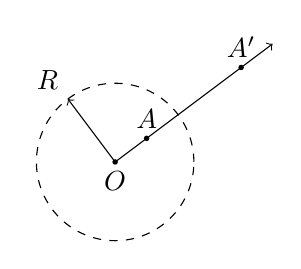
\begin{tikzpicture}
          \draw[dashed] (0, 0) circle (1);
          \draw[->] (0, 0) -- (-0.6, 0.8)  node[above left] { $R$ };
          \draw[->] (0, 0) -- (2, 1.5);
          \fill (0.4, 0.3) circle (1pt) node[above] {$A$};
          \fill (1.6, 1.2) circle (1pt) node[above] {$A'$};
          \fill (0, 0) circle (1pt) node[below]{$O$};
    \end{tikzpicture}\]
    }
    \note{
    Инверсия --- инволюция, то есть $I^2 = \id$
    }
    \theorem{\label{inversion}
        Инверсия --- конформное отображение, его конформный фактор в точке $A$ равен $\lambda(A) = \frac{R^2}{|OA|^2}$.
    При инверсии плоскости окружности и прямые переходят в окружности и прямые.
    \provenumbers{
    \item[2.] Сначала покажем, что окружности и прямые переходят в окружности и прямые.
        На рисунках $O$ --- центр инверсии, а образы точек при инверсии называются теми же буквами с добавлением штриха.
        \begin{figure}[!ht]
            \begin{minipage}{0.5\textwidth}
                \[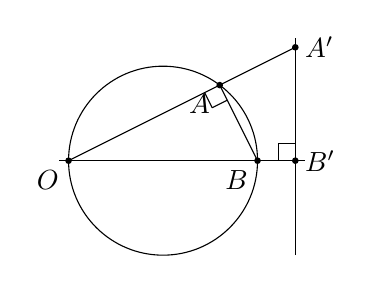
\begin{tikzpicture}[scale=1.2]
              \draw (0, 0) circle (1);
              \draw (1.4, -1) -- (1.4, 1.3);
              \draw (-1, 0) -- (1.4, 1.2);
              \draw (-1.1, 0) -- (1.5, 0);
              \fill (0.6, 0.8) circle (1pt) node[below left] {$A$};
              \fill (1, 0) circle (1pt) node[below left] {$B$};
              \fill (1.4, 0) circle (1pt) node[right] {$B'$};
              \fill (1.4, 1.2) circle (1pt) node[right] {$A'$};
              \fill (-1, 0) circle (1pt) node[below left]{$O$};
              \draw (1, 0) -- (0.6, 0.8);
              \draw (0.6 + 0.08, 0.8 - 0.16) -- (0.6 - 0.08, 0.8 - 0.24);
              \draw (0.6 - 0.16, 0.8 - 0.08) -- (0.6 - 0.08, 0.8 - 0.24);
              \draw (1.22, 0) -- (1.22, 0.18);
              \draw (1.22, 0.18) -- (1.4, 0.18);
        \end{tikzpicture}\]
                \end{minipage}
                \begin{minipage}{0.5\textwidth}
                    \[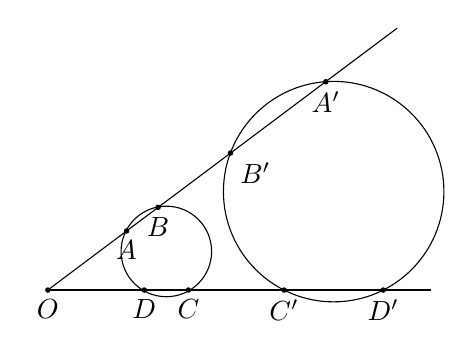
\begin{tikzpicture}[scale=0.5]
                          \fill (0, 0) circle (2pt)  node[below] {$O$};
                          \fill (2.45, 0) circle (2pt)  node[below] {$D$};
                          \fill (3.57, 0) circle (2pt)  node[below] {$C$};
                          \fill (2, 1.5) circle (2pt)  node[below] {$A$};
                          \fill (2.8, 2.1) circle (2pt)  node[below] {$B$};
                          \fill (8.52, 0) circle (2pt)  node[below] {$D'$};
                          \fill (6, 0) circle (2pt)  node[below] {$C'$};
                          \fill (7.06, 5.29) circle (2pt)  node[below] {$A'$};
                          \fill (4.64, 3.48) circle (2pt)  node[below right] {$B'$};
                          \draw (7.26, 2.5) circle (2.8);
                          \draw (3.01, 0.98) circle (1.15);
                          \draw (0, 0) -- (9.73, 0);
                          \draw (0, 0) -- (8.87, 6.65);
                    \end{tikzpicture}\]
                    \end{minipage}
            \end{figure}
    \bullets{
    \item На левом рисунке показано, как окружность, проходящая через центр инверсии, переходит в прямую: если $OB$ --- диаметр окружности, то прямая, перпендикулярная $OB$, и проходящая через $B'$ --- образ окружности.
        В самом деле, для любой пары точек $A$ и $A'$ треугольники $OAB$ и $OB'A'$ подобны;\ угол $OAB$ прямой, если и только если $A$ на окружности, а угол $OB'A'$ прямой, если и только если $A'$ на прямой.
        \item На правом рисунке изображены точки $A, B, C, D$, лежащие на окружности, не содержащей ни внутри себя, ни на границе, центра инверсии.
        Тогда (ссылка на факт из школьной геометрии) $|OA| \cdot |OB| = |OC| \cdot |OD|$, применяя определение инверсии получаем $|OA'| \cdot |OB'| = |OC'| \cdot |OD'|$, откуда (применяя обратный факт) точки $A', B', C', D'$ тоже лежат на одной окружности.
        \item Случай, когда центр инверсии лежит внутри одной из окружностей аналогичен предыдущему, тогда центр инверсии лежит внутри и образа этой окружности.
    \item Наконец, прямая, проходящая через центр инверсии, при инверсии переходит в себя.
    }
    \item[1.] Для проверки, что $\lambda(A) = \frac{R^2}{|OA|^2}$, достаточно рассмотреть все плоскости, содержащие прямую $OA$.
        Пусть $\gamma_1$ --- параметризация одномерной окружности радиуса $OA$, $\gamma_1(0) = A$, и $\gamma_2$ --- параметризация луча $OA$, $\gamma_2(0) = A$:
    \[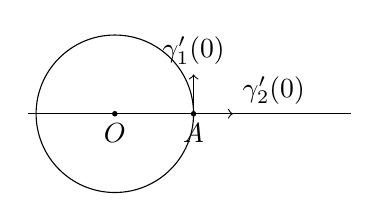
\begin{tikzpicture}
          \draw (0, 0) circle (1);
          \draw (-1.1, 0) -- (3, 0);
          \fill (0, 0) circle (1pt) node[below] {$O$};
          \fill (1, 0) circle (1pt) node [below] {$A$};
          \draw[->] (1, 0) -- (1.5, 0) node[above right] {$\gamma_2'(0)$};
          \draw[->] (1, 0) -- (1, 0.5) node[above] {$\gamma_1'(0)$};
    \end{tikzpicture}\]
    Векторы $\gamma_1'(0)$ и $\gamma_2'(0)$ образуют базис $T_A\R^2$.
    Применим инверсию к картинке.
    \bullets{
        \item $(I \circ \gamma_1)(t) = \frac{R^2}{|OA|^2}\gamma_1(t)$, откуда $\abs{(I \circ \gamma_1)'(0)} = \frac{R^2}{|OA|^2}\abs{\gamma_1'(0)}$.
        \item $(I \circ \gamma_2)(t) = \frac{R^2}{|\gamma_2(t)|^2}\gamma_2(t)$, откуда $\abs{(I \circ \gamma_2)'(0)} = \abs{\frac{\d}{\d t}\big|_{t=0}\frac{R^2}{|\gamma_2(t)|}} = \frac{R^2}{|OA|^2}\cdot\abs{\gamma_2'(0)}$.\qedhere
    }
    }
    }
    \note{Стереографическая проекция --- сужение инверсии --- сохраняет углы.}
    В модели плоскости Лобачевского в верхней полуплоскости имеется \emph{абсолют} --- прямая $\defset{(x, y) \subset \R^2}{y = 0}$.
    \definition[Изометрия]{
    Диффеоморфизм, сохраняющий метрику ($|\_|$ или $\angles{\_,\_}$ --- достаточно что-то одно из двух).
    }
    \theorem{\label{motions}
    Следующие отображения --- изометрии плоскости Лобачевского:
    \numbers{
    \item Сдвиг $S_c: (x, y) \mapsto (x + c, y)$.
    \item Отражение $R_c: (x, y) \mapsto (2c - x, y)$.
    \item Гомотетия с центром на абсолюте и положительным коэффициентом.
    \item Инверсия с центром на абсолюте.
    }
    \provehere{
    Надо просто проверить, что данные отображения сохраняют $|\_|$.
    \numbers{
    \item[1., 2.] Очевидно.
    \item[3.] Такая гомотетия сопряжена при помощи сдвига гомотетии с центром в $(0, 0)$.
    Пусть $f: (x, y) \mapsto (kx, ky)$, тогда $\forall v \in T_{(x_0, y_0)}\H^2: \abs{\d_{(x_0,y_0)} f(v)}_E = k |v|_E$, и так как конформный фактор в $(kx_0, ky_0)$ в $k$ раз меньше фактора в $(x_0, y_0)$, то действительно $\abs{\d_{(x_0,y_0)} f(v)}_{\H} = |v|_{\H}$.
    \item[4.] В силу доказанного выше, достаточно проверить для инверсии с центром в $O = (0, 0)$ и радиусом $R = 1$.
    Такая инверсия действует по правилу $I: (x_0, y_0) \mapsto \left(\frac{x_0}{r^2}, \frac{y_0}{r^2}\right)$, где $r = \sqrt{x_0^2 + y_0^2}$.
    Согласно~(\cref{inversion}), в евклидовой метрике $\forall v \in T_{(x_0, y_0)}\H^2: \abs{\d_{(x_0,y_0)}I(v)}_E = \frac{1}{r^2}|v|_E$.
    Получаем
    \[|\d_{(x_0,y_0)}I(v)|_{\H} = \frac{|\d_{(x_0,y_0)}I(v)|_E}{\nicefrac{y_0}{r^2}} = \frac{|v|_{E}}{y_0} = |v|_{\H}\qedhere\]
    }
    }
    }
    \definition[Движение плоскости Лобачевского]{
    Изометрия плоскости Лобачевского, получаемая композицией пунктов (1 -- 4) из~(\cref{motions}).
    }
    Когда-нибудь докажем, \comment{или нет}, что других изометрий у плоскости Лобачевского нет.

    Плоскость Лобачевского удобно представлять, как $\C_+ \bydef \defset{z \in \C}{\Im z > 0}$.
    В этом случае все движения записываются в виде
    \[\all{z \mapsto \frac{az + b}{cz + d},&\text{ где }a,b,c,d \in \R, ad - bc > 0 \\ z \mapsto \frac{a\overline{z} + b}{c\overline{z} + d},&\text{ где }a,b,c,d \in \R, ad - bc < 0}\]
    Так как $I(z) = \frac{1}{\overline{z}}$, то несложно проверить, что это группа, и (1 -- 4) из~(\cref{motions}) --- её образующие.

    \definition[Прямые в плоскости Лобачевского]{
    Прямые, перпендикулярные абсолюту, и окружности, перпендикулярные абсолюту (то есть с центром на нём).
    }
    \theorem{
    Через любые две точки плоскости Лобачевского проходит единственная \emph{прямая}, и её отрезок реализует кратчайшее расстояние между данными точками.
    \provehere{
    При движении прямые переходят в прямые, поэтому достаточно доказать эту теорему для случая двух точек, находящихся на одной вертикальной прямой.
    В самом деле, несложно построить окружность с центром на абсолюте, проходящую через две данные точки, и инверсией перевести её в вертикальную прямую.

    Итак, через две точки $(x_0, y_1)$ и $(x_0, y_2)$ очевидным образом проходит всего одна прямая --- вертикальная евклидова прямая.
    Если кусочно-гладкий путь $\gamma(t) = (x(t), y(t))$ соединяет данные точки, то его длина равна $\sum\limits_{i = 0}^{N-1}\int\limits_{t_i}^{t_{i+1}}\frac{\sqrt{\dot{x}^2 + \dot{y}^2}{|y|}}\d t \ge \sum\limits_{i = 0}^{N-1}\int\limits_{t_i}^{t_{i+1}}\frac{\dot{y}{|y|}}\d t$, и равенство наблюдается только при $x' \equiv 0$.
    Иными словами, любой путь при проекции на прямую $x = x_0$ не увеличивает свою длину, причём понятно, что путь будет кратчайшим, если он монотонный.
    }
    }
    \newlection{20 марта 2024 г.}
    \subsection{Аксиомы плоскости Лобачевского}
    <<На самом деле, аксиом много, и их можно по-разному выбирать>>

    Аксиомы аналогичны евклидовым, выпишем некоторые из них:
    \numbers{
    \item Через любые две точки проходит единственная прямая (евклидова окружность с центром на абсолюте или вертикальная прямая).
    \item Прямая разбивает плоскость на две части: любой отрезок, соединяющий две точки, пересекает данную прямую не более, чем в одной точке, и точки бьются на два класса эквивалентности относительно данного отношения.
    \item Аксиома параллельных не верна: через одну точку можно провести много прямых, параллельных данной (не пересекающих данную).

        На данной картинке синим нарисованы некоторые прямые, проходящие через точку $p$, не пересекая данную зелёную прямую $l$:
        \[\begin{tikzpicture}
            \draw[darkgreen,thick] (0, 0) -- (0, 2) node[above right] {$l$};
            \fill (1.5, 0.5) circle (1pt) node[above right] {$p$};

            \draw[blue,thick] (2, 0) circle ({sqrt(2)/2});
            \draw[blue,thick] (1, 0) circle ({sqrt(2)/2});
            \draw[blue,thick] (1.5, 0) -- (1.5, 2);
            \fill[white] (0, 0) rectangle (2.9, -1);
            \draw[->] (-1, 0) -- (3, 0) node[above right]{$x$};

        \end{tikzpicture}\]

    \intfact{Это равносильно тому, что не существует точки $O$, в которой можно произвести гомотетию, то есть такое отображение $H: \H^2 \map \H^2$ с коэффициентом $\lambda \in \R$, что $H(O) = O, d(H(A), H (B)) = \lambda d(A, B)$.}
    \item Однородность движения.
    \definition[Флаг]{Тройка из точки, луча и полуплоскости, расположенных так:
    \[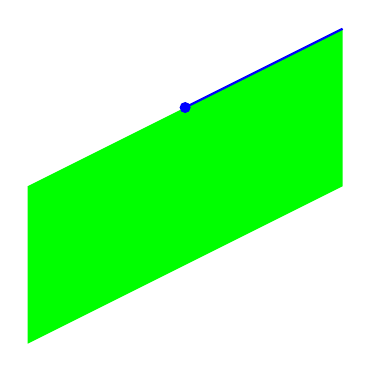
\begin{tikzpicture}
          \fill[green] (-2,-1) -- (2,1) -- (2, -1) -- (-2,-3) -- cycle;
          \draw[blue,thick] (0, 0) -- (2, 1);
          \fill[blue] (0,0) circle (2pt);
    \end{tikzpicture}\]
    Говоря словами, берётся точка, из прямой (в смысле гиперболической плоскости --- евклидова прямая либо окружность), проходящей через данную точку, оставляется только одна половина --- луч, и так как прямая делит плоскость на две части, то также выбирается одна из частей --- полуплоскость.

    Аксиома однородности движения говорит, что любой такой флаг (набор из точки, луча и полуплоскости), переводится в любой другой флаг движением.
    }
    \proposal{
        Докажем, что данная аксиома верна в нашей модели.
    \provehere{
        Достаточно доказать, что в данный флаг можно перевести любой другой.

        В качестве фиксированного флага выберем флаг $[(0, 1), \text{вверх}, \text{вправо}]$:
        \[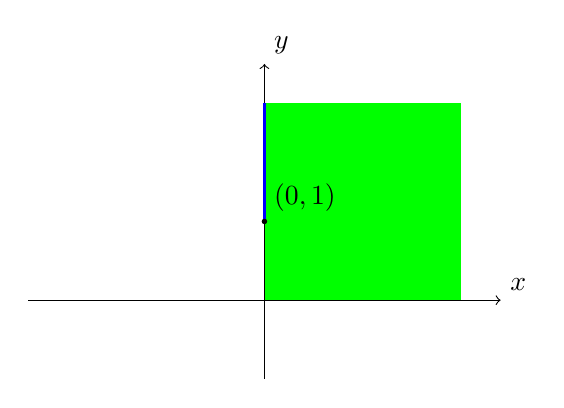
\begin{tikzpicture}
              \fill[green] (0, 0) rectangle (2.5, 2.5);
              \draw[->] (-3, 0) -- (3, 0) node[above right] {$x$};
              \draw[->] (0, -1) -- (0, 3) node[above right] {$y$};
              \draw[blue, very thick] (0, 1) -- (0, 2.5);
              \fill (0, 1) circle (1pt) node [above right] {$(0, 1)$};
        \end{tikzpicture}\]

        Рассмотрим другой флаг, характеризующийся точкой $p$, и выберем на луче другую точку $q$.
    Пусть $d \coloneqq d(p, q)$.
        Переведём точки $p$ и $q$ в точки $(0, 1)$ и $(0, e^d)$ соответственно:
    \bullets{
    \item Если $p$ и $q$ не лежат на одной вертикальной прямой, то прямая, проходящая через них --- евклидова окружность с центром на абсолюте.
    Пусть она пересекает абсолют в точке $X$ (и ещё какой-то), сделав инверсию в $X$, мы сведёмся к следующему случаю.
    \item Теперь $p$ и $q$ лежат на одной вертикальной прямой, пересекающей абсолют в точке $Y$.
    Если $p$ выше $q$, то сделаем инверсию в $Y$, теперь $p$ ниже $q$.
    \item Далее гомотетией с центром в $Y$ переведём $p$ в $(0, 1)$. Так как все проделанные преобразования --- изометрии, а последняя сохраняет вертикальную прямую $pq$, то $q$ перейдёт в точку $(0, e^d)$.
    \item Чтобы совместить флаги, осталось, если нужно, сделать отражение относительно прямой $x = 0$ (точки и лучи уже совмещены, но надо ещё совместить полуплоскости).\qedhere
    }
    }}
    \item Неравенство треугольника: $d(x, y) \le d(x, z) + d(z, y)$, и равенство имеет место только когда $z \in [x, y]$ (разумеется, отрезок --- множество точек гиперболической прямой $xy$, лежащих между $x$ и $y$).
    }
    \subsection{Модель Пуанкаре в круге}
    Обозначим модель Лобачевского в верхней полуплоскости $\H_L$.
    Сделаем инверсию $I$ модели Лобачевского относительно $A = (0, -1)$ с коэффициентом $K = \sqrt{2}$.

    Абсолют $y = 0$ перешёл в окружность, проходящую через точки $(0, 1)$ (образ $(0, 0)$) и $(0, -1)$ (образ бесконечно удалённой).
    Из симметрии относительно прямой $x = 0$ получаем, что абсолют перешёл в окружность $\omega \coloneqq \defset{(x, y)}{x^2+y^2=1}$.

    Данная модель, получающаяся при инверсии модели Лобачевского в верхней полуплоскости, называется \emph{моделью Пуанкаре в круге}, обозначим её $\H_P$.
    Так как инверсия конформна, а $\angles{v, w}_{\H_P} = \angles{\d I(v), \d I(w)}_{\H_L}$, то метрика осталась конформной.

    Роль прямых теперь играют диаметры $\omega$ и дуги окружностей, ортогональных $\omega$ (инверсия сохраняет углы, а все прямые ортогональны абсолюту).
    \theorem{
    Конформный фактор метрики равен $\frac{2}{1 - x^2 - y^2}$.
    Иными словами, для $v \in T_{(x, y)}\H_P: |v|_{\H_P} = \frac{2}{1 - x^2 - y^2}|v|_E$.
    \provehere{
         Рассмотрим $(x_0, y_0) \in \H_P$.
        Пусть $(x_1, y_1) = I(x_0, y_0)$.
        Конформный фактор гиперболической плоскости в модели Лобачевского в точке $(x_1, y_1)$ равен $\frac{1}{y_1}$.

        Пусть при инверсии с центром в точке $A = (0, -1)$ точка $B$ переходит в $B'$.
        Тогда имеется равенство $\dir{AB} = \dir{AB'}\frac{R^2}{|AB'|^2}$.
        Выразим $y_1$ через $x_0, y_0$ (здесь $r = \sqrt{x_0^2 + (y_0 + 1)^2}$):
        \[y_1 = -1 + (y_0 + 1) \cdot \frac{2}{x_0^2 + (y_0 + 1)^2} = \frac{-x_0^2 - y_0^2 + 1}{r^2}\]
        С другой стороны, конформный фактор инверсии равен $\lambda_I = \frac{2}{r^2}|v|_E$.

        Получаем для $v \in T_{(x_0, y_0)}\H_P$: так как инверсия $I$ сохраняет метрику (мы просто так определили метрику на $\H_P$), то $|v|_{\H_P} = |\d_{(x_0, y_0)} I(v)|_{\H_L} = \frac{|\d I(v)|_E}{y_1} = \frac{2}{1 - x_0^2 - y_0^2} |v|_E$.

    Можно записать теперь, что матрица Грама имеет вид $\vect{\frac{4}{(1 - x^2 - y^2)^2}&0\\0&\frac{4}{(1 - x^2 - y^2)^2}}$.
    }
    }
    \comment{Теперь несложно проверить, что никаких изометрий плоскости Лобачевского, кроме объявленных в~(\cref{motions}) нет.
    Так как движения действуют транзитивно на флагах, то достаточно увидеть, что движения содержат стабилизатор любого флага (здесь применяется лемма о действии групп, доказанная в курсе комплексного анализа при изучении автоморфизмов $\hat{\C}$).
    При этом всякая изометрия, оставляющая в модели Пуанкаре центр круга $(0, 0)$, оставляет на месте и все окружности $x^2 + y^2 = r^2$ для $r \in (0, 1)$.
    Рассмотрим изометрии, стабилизирующие следующий флаг:}
    \[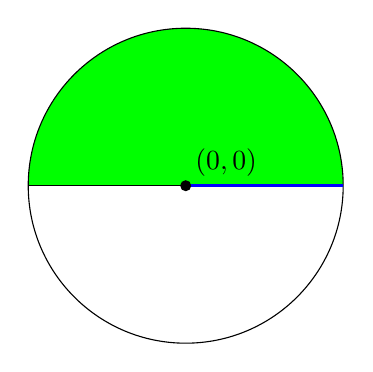
\begin{tikzpicture}
          \fill[green,smooth,domain=0:180] plot ({2 * cos(\x)}, {2 * sin(\x)});
          \draw (0, 0) circle (2);
          \draw (-2, 0) -- (2, 0);
          \draw[blue,very thick] (0, 0) -- (2, 0);
          \fill (0, 0) circle (2pt) node[above right] {$(0, 0)$};
    \end{tikzpicture}\]

    \comment{Рассмотрим окружность $x^2 + y^2 = \frac{1}{2}$.
    Она изометрична евклидовой окружности (конформный фактор во всех точках одинаков), очевидно, что любая изометрия, стабилизирующая данный флаг, действует на ней тождественно.
    }

    \comment{Так как изометрия сохраняет прямые, в частности, диаметры окружности $x^2 + y^2 = 1$, то изометрия, тождественно действующая на окружности $x^2 + y^2 = \frac{1}{2}$ тождественно действует на всём круге.
    Тем самым, стабилизатор каждой точки тривиален, то есть движения совпадают с изометриями.}
    \section{Касательный вектор как дифференцирование}
    Пусть $M$ --- гладкое многообразие. $\mathscr{F}(M)$ --- множество гладких функций $M \map \R$, $\mathscr{X}(M)$ --- множество гладких векторных полей.

    Естественным образом, $\mathscr{F}(M)$ и $\mathscr{X}(M)$ образуют векторные пространства над $\R$.
    При этом, на $\mathscr{F}(M)$ также есть поточечное умножение, и $\mathscr{F}(M)$ таким образом формируют ассоциативную, коммутативную $\R$-алгебру.
    А ещё $\mathscr{X}(M)$ также является модулем над $\mathscr{F}(M)$ --- относительно поточечного умножения.

    Как известно из курса алгебры, дифференциальный оператор $D$ на $\R$-алгебре $A$ --- это такой $\R$-линейный оператор $D: A \map A$, что выполнено правило Лейбница: $D(f \cdot g) = D(f) \cdot g + f \cdot D(g)$.
    Все дифференцирования образуют $\R$-линейное пространство $\Der(A)$.

    Для алгебры $\mathscr{F}(M)$ всякий $X \in \mathscr{X}(M)$ индуцирует дифференцирование $D_X$:
    \[f \in \mathscr{F}(M) \mapsto D_X(f) \in \mathscr{F}(M) \text{, определённый так: }(D_X(f))(x) = \d_x f(X_x)\]
    Правило Лейбница выполнено, так как оно имеет место при дифференцировании произведения.
    \fact{Отображение $\mathscr{X}(M) \map \Der(\mathscr{F}(M)), X \mapsto D_X$ --- гомоморфизм $\R$-векторных пространств.
    \provehere{Несложно проверить.}}
    Далее применение дифференцирования, индуцированного векторным полем $X$, к функции $f$ обозначается просто $X(f)$.
    \theorem{
    Выше определённое отображение $\mathscr{X}(M) \map \Der(\mathscr{F}(M))$ является изоморфизмом.
    \provehere{
     \indentlemma{
         Зафиксируем $p \in M$.

            Пусть $\overline{D}: \mathscr{F}(M) \map \R$ --- $\R$-линейное отображение, такое, что $\overline{D}(f \cdot g) = \overline{D}(f) \cdot g(p) + f(p) \cdot \overline{D}(g)$.
         Например, подходит отображение <<продифференцировать вдоль данного вектора и взять значение в точке $p$>>.
    \numbers{
        \item Тогда $\exists ! v \in T_p M: \overline{D} = D_v \bydef [f \mapsto \d_p f(v)]$.
        \item Несложно получить координаты этого вектора $v$.
        Рассмотрим карту $(U, \phi)$, содержащую точку $p$. В $\R^n$ есть координаты $x_1, \dots, x_n$, пусть $(\tilde{x}_i)_{i=1}^{n} \subset \mathscr{F}(M)$ --- функции, отвечающие координатам ($\tilde{x}_i = x_i \circ \phi$).

        Утверждается, что $v_i = \overline{D}(\tilde{x}_i)$.
    }
    }{
         Заметим, что $\overline{D}(\const) = 0$ (проверим для $f \equiv 1: \overline{D}(1) = \overline{D}(1) \cdot 1 + 1 \cdot \overline{D}(1) = 2\overline{D}(1)$).

         Далее проверим, что $\overline{D}$ локально: если $f\big|_{U_p} = g\big|_{U_p}$, то $\overline{D}(f) = \overline{D}(g)$.
         Сконструируем такую <<шапочку>> $h \in \mathscr{F}(M)$, что $h(p) = 1$, и $h\big|_{M \sm U_p} \equiv 0$.
         Для проверки локальности заметим, что $f\big|_{U_p} = g\big|_{U_p} \iff f \cdot h = g \cdot h$.
         Выкладка
         \[\overline{D}(f \cdot h = g \cdot h) = \all{\overline{D}(f) \cdot h(p) + f(p) \cdot \overline{D}(h)\\ \overline{D}(g) \cdot h(p) + g(p) \cdot \overline{D}(h)}\]
        показывает локальность.

        Теперь убедимся, что такой вектор $v \in T_p M$, если существует, то единственен.
        Для этого проверим равенства во втором пункте, явно задающие координаты $v$.
        Пусть $\phi$ --- карта, $v = (v_1, \dots, v_n)$. Так как $D_v(\tilde{x}_i) = v_i$, то отсюда следует второй пункт.

        Теперь докажем существование такого вектора $v \in T_p M$.
         Зафиксируем карту $(U, \phi)$, содержащую $p$.
         Положим $v_i \coloneqq \overline D(E_i)$, и убедимся, что вектор $(v_1, \dots, v_n)$ задаёт $\overline{D}$.
        \indentlemma[Адамар]{
            Пусть $f \in C^{\infty}(\R^n)$. Тогда $\exists g_1, \dots, g_n$ --- гладкие, такие, что $f(x) - f(0) = \sum\limits_{i}g_i(x) \cdot x_i$.
        }{
            Положим $g_i(x) \coloneqq \int\limits_{0}^{1}\der{f}{x_i}(tx)\d t$.
            Они подходят:
        \[f(x) - f(0) = \int\limits_{0}^{1}\frac{\d}{\d t} f(tx)\d t =  \int\limits_{0}^{1}\sum\limits_{i = 1}^{n}\der{f}{x_i}(tx)\cdot x_i \d t = \sum\limits_{i = 1}^{n}g_i(t)\cdot x_i\qedhere\]
        }
%        Отождествим при помощи диффеоморфизма $\phi$ карту $U \subset M$ и её образ $\phi(U) \subset \R^n$.
%         Можно считать, что $\phi(p) = 0$.
%
%            Выберем $f \in C^{\infty}(\R^n)$, применим лемму Адамара, получим функции $g_i \in C^{\infty}(\R^n)$, такие, что $f(x) = f(0) + \sum\limits_{i = 1}^{n}g_i(x)x_i$ в окрестности $0$.
%         Теперь распишем \begin{multline*}\overline{D}\left({f}\right) = \overline{D}\left({f}(0) + \sum\limits_{i=1}^{n}{x}_i \cdot {g}_i\right) = \sum\limits_{i=1}^{n}\overline{D}\left({x}_i \cdot {g}_i\right) =\\= \sum\limits_{i=1}^{n}\overline{D}\left({x}_i\right) \cdot {g}_i + \underbrace{{x}_i}_{=0} \cdot \overline{D}\left({g}\right) = \sum\limits_{i = 1}^{n} v_i \cdot {g}_i\end{multline*}
%     Так как $ g_i = \der{ f}{ x_i}$, то действительно $\overline{D}({f}) = D_v({f})$.


%%%%      Закомментировано чуть менее формальное, но чуть более понятное, рассуждение


         Можно считать, что $\phi(p) = 0 \in \R^n$.
         Выберем $\tilde{f} \in \mathscr{F}(M)$, применим к $f \coloneqq \tilde{f} \circ \phi^{-1} \in C^{\infty}(\R^n)$ лемму Адамара, получим функции $g_i \in C^{\infty}(\R^n)$.
         Обозначим $\tilde{g}_i \coloneqq g_i \circ \phi^{-1}$, получили разложение $\tilde{f}(x) = \tilde{f}(p) + \sum\limits_{i = 1}^{n}\tilde{g}_i(x)\tilde{x}_i$.
         Теперь распишем \begin{multline*}\overline{D}\left(\tilde{f}\right) = \overline{D}\left(\tilde{f}(p) + \sum\limits_{i=1}^{n}\tilde{x}_i \cdot \tilde{g}_i\right) = \sum\limits_{i=1}^{n}\overline{D}\left(\tilde{x}_i \cdot \tilde{g}_i\right) =\\= \sum\limits_{i=1}^{n}\overline{D}\left(\tilde{x}_i\right) \cdot \tilde{g}_i + \underbrace{\tilde{x}_i}_{=0} \cdot \overline{D}\left(\tilde{g}\right) = \sum\limits_{i = 1}^{n} v_i \cdot \tilde{g}_i\end{multline*}
         Так как $\tilde g_i = \der{\tilde f}{\tilde x_i}$, то действительно $\overline{D}(\tilde{f}) = D_v(\tilde{f})$.
        }
    Рассмотрим дифференцирование $D \in \Der(\mathscr{F}(M))$.
        Согласно лемме, $\forall p \in M: \exists !v_p \in T_p M$, такой, что отображение $f \mapsto D(f)(p)$ совпадает с $f \mapsto D_{v_p}(f)$.
    Это показывает инъективность $\mathscr{X}(M) \map \Der(\mathscr{F}(M))$, а для сюръективности надо убедиться, что полученное поле $p \mapsto v_p$ гладкое.

    Проверим гладкость $p \mapsto v_p$ в карте.
        Лемма даёт координатное представление $(v_p)_i = D(\tilde{x}_i)(p)$, это действительно гладкая функция.
    Осталось сказать, что для проверки гладкости достаточно проверить гладкость координат.
    }
    }
    \newlection{27 марта 2024 г.}
    \section{Скобка Ли векторных полей}
    Пусть $M$ --- гладкое многообразие, $X, Y \in \mathscr{X}(M)$.
    \definition[Скобка Ли векторных полей]{
        Отображение $[\_, \_]: \mathscr{X}(M) \times \mathscr{X}(M) \map \mathscr{X}(M)$, сопоставляющее двум полям $X, Y$ векторное поле, отвечающее дифференцированию
        \[X(Y(f)) - Y(X(f))\label{lie-bracket}\tag{$[-]$}\]
    Иными словами, $[X, Y]f = X(Y(f)) - Y(X(f))$.
    }
    Проверим, что~(\ref{lie-bracket}) является дифференцированием.
    Линейность очевидна;\ правило Лейбница говорит, что должно быть равенство такого
    \[[X, Y](f \cdot g) = ([X, Y]f) \cdot g + f \cdot ([X, Y]g) = (X(Y(f)) - Y(X(f))) \cdot g + f \cdot (X(Y(g)) - Y(X(g)))\]
    и такого выражений:
    \multline{[X, Y](f \cdot g) = X(Y(f \cdot g)) - Y(X(f \cdot g))= X(Y(f) \cdot g + f \cdot Y(g)) - Y(X(f) \cdot g + f \cdot X(g)) =\\ X(Y(f)) \cdot g + \cancelwith[red]{Y(f) \cdot X(g)} + \cancelwith[darkgreen]{X(f) \cdot Y(g)} + f \cdot X(Y(g)) - Y(X(f)) \cdot g - \cancelwith[darkgreen]{X(f) \cdot Y(g)} - \cancelwith[red]{Y(f) \cdot X(g)} - f \cdot Y(X(g)) }
    \subsection{Выражение для скобки Ли в координатах}
    \label{coordinate-for-lie-bracket}
    Пусть $X, Y$ --- два гладких векторных поля, $\phi: U \map \Omega$ --- карта.

    Введём $\tilde{x}_i \coloneqq x_i \circ \phi$, запишем (где $X^\phi \bydef \d\phi \circ X \circ \phi^{-1}$ --- векторное поле на $\phi(U) \subset \R^n$)
    \[[X, Y]_i = D_{[X, Y]}(\tilde{x}_i) =D_{[X^\phi, Y^\phi]}(x_i) = [X^\phi, Y^\phi]_i = X^\phi (Y^\phi(x_i)) - Y^\phi (X^\phi(x_i)) = X^{\phi}(Y_i) - Y^{\phi}(X_i) \]
    \subsection{Пространство $\mathscr{X}(M)$ вместе со скобкой Ли, как алгебра Ли}
    Чтобы проверить, что $\mathscr{X}(M)$ образует алгебру Ли, убедимся, что выполнены три аксиомы алгебр Ли:
    \numbers{
    \item Линейность по обеим аргументам: $\forall \alpha_i, \beta_j \in \R, X, Y \in \mathscr{X}(M)$: \gather{[\alpha_1 X_1 + \alpha_2 X_2, Y] = \alpha_1[X_1, Y] + \alpha_2[X_2, Y] \\ [X, \beta_1 Y_1 + \beta_2 Y_2] = \beta_1[X, Y_1] + \beta_2[X, Y_2]}
    \item Кососимметричность: $[X, Y] = -[Y, X]$, или же (эквивалентно) антисимметричность ${[X, X] = 0}$.
    \item Тождество Якоби $[X, [Y, Z]] + [Y, [Z, X]] + [Z, [X, Y]] = 0$.
    }
    Все три свойства следуют из того, что изоморфизм $\R$-векторных пространств $\mathscr{X}(M) \map \Der(\mathscr{F}(M))$ сохраняет скобку Ли (просто по определению скобки Ли на $\mathscr{X}(M)$).
    То, что для любой алгебры $A$: $\Der(A)$ --- алгебра Ли --- известный факт.
    Проверим тождество Якоби: $\forall X, Y, Z \in \Der(A), \forall a \in A$:
    \multline{[X, [Y, Z]](a) = X([Y, Z](a)) - [Y, Z](X(a)) =\\= X(Y(Z(a))) - X(Z(Y(a))) - Y(Z(X(a))) + Z(Y(X(a)))}
    Записывая аналогичные равенства для $[Y, [Z, X]]$ и $[Z, [X, Y]]$, и складывая, получим $0$ --- всё сократится.
    \subsection{Специфичные свойства скобки Ли векторных полей}
    Пусть $f, g \in \mathscr{F}(M)$.
    \properties[Скобка Ли векторных полей]{
    \item $[f\cdot X, Y] = f \cdot [X, Y] - Y(f) \cdot X$.
        \provehere{Применим к $h \in \mathscr{F}(M)$:
        \[[f\cdot X, Y](h) = (f\cdot X)(Y(h)) - Y((f\cdot X)(h)) =(f\cdot X)(Y(h)) - Y(f \cdot X(h))\circlesign{=}\]
        Так как $(f\cdot X)(\cdots)$ --- это производные по направлению, то это равно $f \cdot X(\cdots)$.
        \[\circlesign{=}f \cdot (X(Y(h))) - Y(f) \cdot X(h) - f \cdot Y(X(h))\qedhere\]
        }
    \item $[X, g\cdot Y] = g \cdot [X, Y] + X(g) \cdot Y$.
        \provehere{
        Ради разнообразия, выведем из первого и кососимметричности
        \[[X, g\cdot Y] = -[g\cdot Y, X] = -(g \cdot [Y, X] - X(g) \cdot Y) = g \cdot [X, Y] + X(g) \cdot Y\qedhere\]
        }
    \item $[f\cdot X, g \cdot Y] = f\cdot g\cdot[X, Y] + f\cdot X(g) \cdot Y - g(Y(f)) \cdot X$.
    \provehere{
    \[[f\cdot X, g\cdot Y] = g \cdot [f\cdot X, Y] + (f \cdot X)(g) \cdot Y = g \cdot (f \cdot [X, Y] - Y(f) \cdot X) + (f \cdot X)(g) \cdot Y\qedhere\]
    }
    }
    \definition[Группа Ли]{
    Гладкое многообразие, являющееся топологической группой: умножение $G \times G \map G$ и взятие обратного $G \map G$ --- гладкие отображения.
    }
    \example[Группы Ли]{
    Различные линейные группы: $GL(n, \R), SL(n, \R), O(n, \R), \dots$
    }
    Всякий элемент $g \in G$ действует на группе левыми и правыми трансляциями: $L_g: x \mapsto gx, R_g: x \mapsto xg$.
    \definition[Левоинвариантное векторное поле $X$]{
        Такое поле, что $\forall g \in G: \d L_g(X) = X$.
    }
    Выберем ортонормированный базис $(x_1, \dots, x_n) \in T_1(G)$ ($1 \in G$ --- единица в группе), и распространим $x_1, \dots, x_n$ до левоинвариантных векторных полей $X_1, \dots, X_n$ соответствующим дифференциалом $L_g$ (действие транзитивно, поэтому, $X_1, \dots, X_n$ определены всюду).
    Это будут векторные поля, отвечающие за ортонормированные базисы во всех точках группы.

    Можно определить левоинвариантную метрику: для $\tilde{X}, \tilde{Y} \in T_g(G): \langle\tilde{X}, \tilde{Y}\rangle = \angles{\d_1 L_g(X), \d_1 L_g(Y)}$.
    \section{Тензоры на многообразии}
    Пусть $V$ --- векторное пространство.
    \definition[Тензор типа $(k, m)$]{
    Тензор $\underbrace{(V^* \otimes \cdots \otimes V^*)}_{k} \otimes \underbrace{(V \otimes \cdots \otimes V)}_{m}$
    }
    Мы будем рассматривать только тензоры типа $(k, 0)$ и $(k, 1)$, что, как известно, можно рассматривать, как полилинейные отображения
    \[\underbrace{V \times \dots \times V}_{k} \map \R \text{\quadи\quad}\underbrace{V \times \dots \times V}_{k} \map V\text{\quad соответственно}\]
    Далее в качестве $V$ выступает касательное пространство к данной точке.
    \definition[Тензор (тензорное поле) на $M$ типа $(k, 0)$]{
    Семейство $\{F_x\}_{x \in M}$ тензоров валентности $(k, 0)$ вместе со следующим условием гладкости:
    \[\forall X_1, \dots, X_k \in \mathscr{X}(M): F(X_1, \dots, X_k) \in \mathscr{F}(M)\]
    }
    \example[Тензор типа $(2, 0)$]{
    \item Риманова метрика на $n$-мерном многообразии. %\comment{Так, стоп, это же тензор типа $(2, 0)$, разве нет?}
    }
    \counterexample[Не тензор]{
    \item Символ Кристоффеля $\Gamma_{i,j}^{k}$ не является записью какого-то тензора в координатах:
    отображение $F(X, Y) = \nabla_X Y$ не $\mathscr{F}(M)$-линейно: $\nabla_X(f \cdot Y) = X \cdot f + f \cdot \nabla_X(Y)$.
    }
    \definition[Тензор (тензорное поле) на $M$ типа $(k, 1)$]{
    Семейство $\{F_x\}_{x \in M}$ тензоров валентности $(k, 1)$ вместе со следующим условием гладкости:
    \[\forall X_1, \dots, X_k \in \mathscr{X}(M): F(X_1, \dots, X_k) \in \mathscr{X}(M)\]
    }
    Таким образом, тензорному полю на $M$ сопоставляется $\R$-полилинейное
    \[F: \mathscr{X}(M) \times \dots \times \mathscr{X}(M) \map \any{\mathscr{F}(M) \\ \mathscr{X}(M)}\]
    Несложно видеть, что это отображение даже $\mathscr{F}(M)$-полилинейное (проверяется поточечно), но оказывается, что этого требования достаточно для определения тензора.
    \theorem{\label{tensor}
    Если отображение $F: \mathscr{X}(M) \times \dots \times \mathscr{X}(M) \map \any{\mathscr{F}(M) \\ \mathscr{X}(M)}$ является $\mathscr{F}(M)$-полилинейным, то $F$ однозначно определяет соответствующее гладкое тензорное поле.
    \provehere{
        Сначала докажем случай $k = 1$, то есть $F: \mathscr{X}(M) \map \any{\mathscr{F}(M) \\ \mathscr{X}(M)}$ --- $\mathscr{F}(M)$-линейное отображение.
        \bullets{
            \item Чтобы извлечь из $F$ тензор в данной точке, сначала проверим локальность.

            Рассмотрим $p \in U$.
            Пусть $X, Y \in \mathscr{F}(M)$, причём $X\big|_{U} = Y\big|_U$.
            Рассмотрим $h$ --- гладкий спуск с единицы в $U$: $h\big|_{U'} \equiv 1, h\big|_{M \sm U} \equiv 0$, где $p \in U' \subset U$. \comment{Вместо $h\big|_{U'} \equiv 1$ достаточно потребовать $h(p) = 1$.}
            Теперь $h \cdot F(X) = F(hX) = F(hY) = h \cdot F(Y)$, откуда получаем $F(Y)(p) = F(X)(p)$.
        \item Достаточно доказать для $X \in \mathscr{X}(M)$, что значение $(F(X))(p)$ зависит только от $X_p$.
        Доказав, мы построим семейство, отвечающее $F$, и оно будет обладать требуемым условием гладкости, так как $F$ бьёт в $\mathscr{F}(M)$ или $\mathscr{X}(M)$.

            Зафиксируем карту $(U, \phi)$, содержащую точку $p$.
            Выберем базис $e_1, \dots, e_n$, ему отвечают координатные векторные поля $E_i$.
            Используя~(\cref{extension-of-coordinates}), можно считать, что $E_i$ определены на всём многообразии.

            Пусть $X \in \mathscr{X}(M)$, разложим его по координатным полям: $X = X_1 E_1 + \dots + X_n E_n$ (равенство выполняется в некоторой окрестности $p$), где $X_i \in \mathscr{F}(M)$.
            Используя локальность, запишем
            \[F(X) = F(X_1 E_1 + \dots + X_n E_n) = X_1 F(E_1) + \dots + X_n F(E_n)\]
            Тем самым, $F(X)(p) = X_1(p) \cdot F(E_1)(p) + \dots + X_n(p) \cdot F_n(E_n)(p)$.
    }
    Если $k \ne 1$, то надо доказать сначала локальность ($\forall p \in U: X_1\big|_U = Y_1\big|_U$ $\then$ $F(X_1, Z_2, \dots, Z_n)(p) = F(Y_1, Z_2, \dots, Z_n)(p)$, и по всем остальным аргументам аналогично), а потом то, что $F(X_1, \dots, X_n)(p)$ зависит только от $X_1(p), \dots, X_n(p)$ по очереди по каждому аргументу.
    Это следует из случая $k = 1$, так как при фиксированных $k - 1$ аргументах $F$ линейно по последнему.
    }
    }
    \newlection{3 апреля 2024 г.}
    Пусть $E_i, E_j$ --- координатные поля.
    \fact{
        $[E_i, E_j] = 0$.
    \provehere{
        Запишем выражение для скобки Ли в координатах в карте:~(\cref{coordinate-for-lie-bracket}):
        \[[X, Y]^{\phi}_i = (Y^\phi_i)'_{X^\phi} - (X^\phi_i)'_{Y_\phi}\]
    При этом $X^{\phi}_i, Y^{\phi}_i$ --- константы, их производные равны нулю.
    }
    }
    Вообще, скобка Ли --- мера некоммутативности векторных полей, что мы докажем позже.
    \subsection{Поведение скобки Ли при отображениях}
    Пусть $M, N$ --- гладкие многообразия, $X \in \mathscr{X}(M), Y \in \mathscr{X}(N)$, $F: M \map N$ -- гладкое.
    \definition[$F$ переводит $X$ в $Y$]{
    $\forall p \in M: \d_p F(X_p) = Y_{F(p)}$.
    }
    Вообще говоря, если дано отображение $F: M \map N$, и векторное поле $X \in \mathscr{X}(M)$, то не всегда найдётся $Y \in \mathscr{X}(N)$ такой, что $X$ переходит в $Y$ (например, $F(p) = F(q)$, и $\d_p F(X_p) \ne \d_p F(X_q)$), а если и найдётся, то может быть не единственно, если $F$ не сюръективно.

    Пусть $F: M \map N$ переводит $X \in \mathscr{X}(M)$ в $Y \in \mathscr{X}(N)$.
    \lemma{\label{action-suffices}
    $F$ переводит $X$ в $Y$ $\iff$ $\forall$ гладкого $f: N \map \R: Y(f) \circ F = X(f \circ F)$.
    \provetwhen{
        $X(f \circ F)(p) = \d_p (f \circ F)(X_p) = (\d_{F(p)} f \circ \d_p F)(X_p) = \d_{F(p)} f(Y_{F(p)}) = (Y(f))(F(p))$.
    }{
        Выберем локально $f \coloneqq x_i$ --- координатная функция.
        \[Y_i(F(p)) = (Y (x_i) \circ F)(p) = X(x_i \circ F)(p) = \d_p(x_i \circ F)(X_p) = (\d_{F(p)} x_i \circ \d_p F)(X_p) = (\d_p F(X))_i(p)\]
        Совпали $i$-е координаты полей, значит, сами поля совпали.
    }
    }
    Если $F$ переводит $X$ в $Y$, то будем писать $F(X) = Y$.
    \theorem{
    Пусть $F: N \map M$ гладкое, $X_1, X_2 \in \mathscr{X}(M), Y_1, Y_2 \in \mathscr{X}(N)$.
        Если $F(X_1) = Y_1$ и $F(X_2) = Y_2$, то $F([X_1, X_2]) = [Y_1, Y_2]$.
    \provehere{
        Пусть $f: N \map \R$ --- произвольная гладкая.
    Проверим, что $F([X_1, X_2])$ и $[Y_1, Y_2]$ одинаково действуют на $f$:
    \multline{
        [Y_1, Y_2](f) \circ F = Y_1(Y_2(f)) \circ F - Y_2(Y_1(f)) \circ F = X_1(Y_2(f) \circ F) - X_2(Y_1(f) \circ F) =\\
        = X_1(X_2(f \circ F)) - X_2(X_1(f \circ F)) =  [X_1, X_2](f \circ F)
    }
    Конечно, $F([X_1, X_2])$ априори даже может быть не определено, но выкладка выше корректна, и согласно~(\cref{action-suffices}), её достаточно для проверки.
    }
    }
    \corollary{
        Пусть $M$ --- гладкое многообразие, $N \subset M$ --- гладкое подмногообразие.

        Если $X, Y \in \mathscr{X}(M)$ касательны к $N$, то и $[X, Y]$ --- касательно к $N$.
    \provehere{Рассмотреть $F = \text{in}$ --- вложение $N \hookrightarrow M$. }
    }
    \section{Аффинные связности}
    Пусть $M$ --- гладкое многообразие
    \definition[Аффинная связность $\nabla$]{
    Отображение \begin{align*}\mathscr{X}(M) \times \mathscr{X}(M) &\map \mathscr{X}(M) \\ V, W &\mapsto \nabla_V W\end{align*} со следующими свойствами:
    \numbers{
    \item $\R$-билинейность.
    \item $\mathscr{F}(M)$-линейность по первому аргументу: $\nabla_{f \cdot V}W = f \cdot \nabla_V W$.
    \item Правило Лейбница по второму аргументу: $\nabla_V(f \cdot W) = V (f)\cdot W + f \cdot \nabla_V W$.
    }
    }
    \examples{
    \item Обычное дифференцирование: на $\R^n$ могут быть заданы векторные поля.
    \item Ковариантная производная на поверхности $\Sigma^2 \subset \R^3$
    \item Покоординатное дифференцирование в карте. $(U, \phi)$ --- карта, $E_i$ --- координатные векторные поля, $Y = \sum\limits_{i = 1}^n Y_i E_i$, тогда $\nabla^{\phi}_Y X (p) = \sum\limits_{i = 1}^n X(Y_i) (p) \cdot E_i = \sum\limits_{i = 1}^n \d_p Y_i(X_p) E_i$% $U \subset \R^n$.
    }
%    Несложно видеть из определения, что аффинные связности образуют $\R$-векторное пространство. Нет!!!
    \theorem[О пространстве связностей]{
        Пусть $M$ --- гладкое многообразие, $\nabla, \tilde{\nabla}$ --- две аффинные связности.
    \numbers{
    \item $\nabla - \tilde{\nabla}$ --- тензор типа $(2, 1)$.
    \item Если $T$ --- тензор типа $(2, 1), \nabla$ --- связность, то $T + \nabla$ --- связность.
    }
    \provebullets{
        \item Достаточно проверить $\mathscr{F}(M)$-линейность по второму аргументу:
    \[\nabla_V(f \cdot W) - \tilde{\nabla}_V(f \cdot W) = \cancel{V(f) \cdot W} + f \cdot \nabla_V W - \cancel{V(f) \cdot W} - f \cdot \tilde{\nabla}_V W\]
    \item Достаточно проверить правило Лейбница:
    \[(\nabla + T)_V(f \cdot W) = f(V) \cdot W + f \cdot \nabla_V W + T(V, f \cdot W) = f(V) \cdot W + f \cdot (\nabla + T)_V(W)\qedhere\]
    }
    }
    \proposal[Локальность аффинной связности]{\label{locality-of-nabla}
    Пусть $\nabla$ --- аффинная связность. $\forall V, W \in \mathscr{X}(M): \nabla_V(W)$ зависит только от $V_p$ и $W$ в окрестности $p$.
    \provehere{
        При фиксированном втором аргументе $\nabla_{\_}(W)$ --- тензор типа $(1, 1)$, значит, зависит только от $V_p$.

        Пусть имеются два поля $W_1, W_2$, совпадающие в окрестности $U_p \ni p$. Пусть $h$ --- гладкий спуск с единицы в окрестности $p$, $h\big|_{U_p^\complement} \equiv 0$.
    \[h \cdot (\nabla_V W_2) + \underbrace{(W_2(h) \cdot V)_p}_{0} = \nabla_{V}(h \cdot W_2) = \nabla_V(h \cdot W_1) = h \cdot (\nabla_V W_1) + \underbrace{(W_1(h) \cdot V)_p}_{0}\qedhere\]
    }
    }
    \corollary{
    Для аффинной связности $\nabla$ и открытого $U \subset M$ имеет смысл говорить о сужении $\nabla\big|_U$.
    }
    Рассмотрим карту $\phi: (U \subset M) \map \R^n$.
    Пусть $\nabla$ -- аффинная связность на $M$, а $\nabla^\phi$ --- покоординатное дифференцирование в карте.
    Тогда $\nabla - \nabla^{\phi}$ --- некоторый тензор $\Gamma$ типа $(2, 1)$.

    Пусть $E_1, \dots, E_n$ --- координатные векторные поля.
    Обозначим $\Gamma_{i,j}\coloneqq\Gamma(E_i, E_j)$.
    \definition[Символы Кристоффеля]{\label{cristo-1}
    $\Gamma_{i,j} = \Gamma(E_i, E_j)$.
    }
    В отличие от символов Кристоффеля прошлого семестра, эти отвечают координатам тензора, и имеют смысл не на всём многообразии, а только в данной карте.
    \subsection{Специальные связности}
    \subsubsection{Симметричная связность}
    \definition[$\nabla$ --- симметричная связность]{Такая аффинная связность $\nabla$, что $\forall X, Y \in \mathscr{X}(M): \nabla_X Y - \nabla_Y X = [X, Y]$.}
    \statement{
    $T \coloneqq \nabla_X Y - \nabla_Y X - [X, Y]$ --- тензор типа $(2, 1)$.
    \provehere{
    Выражение антисимметрично ($\nabla_X X - \nabla_X X - [X, X] = 0$) и $\R$-билинейно.
        Проверим $\mathscr{F}(M)$-билинейность по второму аргументу:
    \multline{\nabla_X (f \cdot Y) - \nabla_{f \cdot Y} X - [X, f \cdot Y] = \cancel{X (f) \cdot Y}+ f \cdot \nabla_X Y - f \cdot \nabla_Y X - (f \cdot [X, Y] + \cancel{X(f) \cdot Y}) =\\= f \cdot (\nabla_X Y - \nabla_Y X - [X, Y])}
    Билинейность по первому аргументу следует из антисимметричности.
    }
    }
    Этот тензор $T$ называется \emph{тензор кручения}.
    \corollary{
    Проверку того, что связность симметрична, достаточно осуществлять на координатных полях.
    Для координатных полей $\nabla_{E_i}E_j - [E_i, E_j]=\nabla_{E_i}E_j = \Gamma_{i,j}$.
        Более того, $\nabla^{\phi}_{E_i}(E_j) = 0$.
        Тем самым, связность симметрична $\iff \Gamma_{i,j} = \Gamma_{j,i}$.
    }
    \subsubsection{Риманова связность}
    Пусть $(M, \angles{\_, \_})$ --- многообразие с римановой метрикой.
    \definition[Риманова связность $\nabla$]{
    Аффинная связность $\nabla$, согласованная с римановой метрикой: $X\angles{Y, Z} = \angles{\nabla_X Y, Z} + \angles{Y, \nabla_X Z}$.
    }
    \statement{
        $S \coloneqq X\angles{Y, Z} - \angles{\nabla_X Y, Z} - \angles{Y, \nabla_X Z}$ --- тензор типа $(3, 0)$.
        \provehere{
            $\R$-полилинейность по всем аргументам и $\mathscr{F}(M)$-линейность по первому очевидны.

        По второму и третьему аргументам симметрично, проверим $\mathscr{F}(M)$-линейность по второму:
        \multline{X\angles{f \cdot Y, Z} - \angles{\nabla_X (f \cdot Y), Z} - \angles{f \cdot Y, \nabla_X Z} =\\= \cancel{X(f) \cdot \angles{Y, Z}} + f \cdot X\angles{Y, Z} - \cancel{\angles{X(f) \cdot Y, Z}} - f\angles{  \nabla_X(Y), Z} - f \angles{ Y, \nabla_{X}Z}\qedhere}
        }
    }
    \corollary{Можно проверять римановость связности только на координатных полях.}
    \subsubsection{Связность Леви-Чивиты}
    \definition[Связность Леви-Чивиты]{
        Симметричная риманова связность.
    }
    \newlection{10 апреля 2024 г.}
    \subsection{Символы Кристоффеля}
    Дадим второе определение, и поймём, что оно совпадает с первым.
    У нас зафиксирована аффинная связность $\nabla$, и карта $(U, \phi)$.
    \definition[Символы Кристоффеля в карте]{
    $\Gamma^{\phi}_{i,j} = \nabla_{E_i}E_j$.
    }
    Опять же, символы первого рода $\Gamma_{i,j;k} \bydef \angles{\Gamma_{i,j}, E_k}$, и символы второго рода --- координаты в разложении: $\Gamma_{i,j} = \sum\limits_{k}\Gamma_{i,j}^{k}E_k$.

    Это совпадает с~(\cref{cristo-1}), так как $\Gamma^{\phi}(E_i, E_j) = \nabla_{E_i}E_j - \underbrace{\nabla^{\phi}_{E_i}E_j}_{0}$.
    \fact{Одни символы Кристоффеля гладкие тогда и только тогда, когда гладкие --- другие.
    \provehere{
    Они выражаются друг через друга и матрицу Грама (координаты метрического тензора): $(g_{n,m})\vect{\Gamma_{i,j}^1 \\ \vdots \\ \Gamma_{i,j}^{n}} = \vect{\Gamma_{i,j;1} \\ \vdots \\ \Gamma_{i,j;n}}$, откуда $\vect{\Gamma_{i,j}^1 \\ \vdots \\ \Gamma_{i,j}^{n}} =(g_{n,m})^{-1} \vect{\Gamma_{i,j;1} \\ \vdots \\ \Gamma_{i,j;n}}$.
    }
    }
    \subsection{Существование и единственность связности Леви-Чивиты}

    \theorem[Основная теорема римановой геометрии]{
        Пусть $(M, \angles{\_,\_})$ --- риманово многообразие.
        Тогда существует и единственна связность Леви-Чивиты $\nabla$.
    \provehere{
%    Сначала докажем единственность: пусть $(U, \phi)$ --- карта, тогда $E_k(\angles{E_i, E_j}) = \angles{\nabla_{E_k}E_i, E_j} + \angles{E_i, \angles_{E_k}E_j}$ согласно римановости.
%
    Зафиксируем карту $(U, \phi)$, в ней имеется $n^2$ гладких функций $g_{i,j}$.
        В силу римановости связности Леви-Чивиты: \[E_k(g_{i,j}) = E_k\angles{E_i, E_j} = \angles{\Gamma_{k,i}, E_j} + \angles{E_i, \Gamma_{k,j}} = \Gamma_{k,i;j} + \Gamma_{k,j;i}\]
    Переставляя индексы циклически, получаем $\all{E_k(g_{i,j}) = \angles{\Gamma_{k,i}, E_j} + \angles{E_i, \Gamma_{k,j}} = \Gamma_{k,i;j} + \Gamma_{k,j;i}\\E_i(g_{j,k}) = \angles{\Gamma_{i,j}, E_k} + \angles{E_j, \Gamma_{i,k}} = \Gamma_{i,j;k} + \Gamma_{i,k;j}\\E_j(g_{k,i}) = \angles{\Gamma_{j,k}, E_i} + \angles{E_k, \Gamma_{j,i}} = \Gamma_{j,k;i} + \Gamma_{j,i;k}}$
    Так как символы симметричны, то есть $\Gamma_{i,j;k} = \Gamma_{j,i;k}$, то
    \[\Gamma_{i,j;k} = \frac{E_j(g_{i,k}) + E_i(g_{j,k}) - E_k(g_{i,j})}{2}\label{gamma-equals-what}\tag{$*$}\]
    Это показывает единственность в каждой карте, значит, и глобальную единственность.

    Докажем существование.
    Зафиксируем карту, и проверим, что выражение через~\eqref{gamma-equals-what} корректно определяет связность Леви-Чивиты формулой $\nabla = \nabla^{\phi} + \Gamma^{\phi}$.
        Симметричность $\nabla$ очевидна (проверяем на базисных векторах).
        По модулю симметричности, римановость в точности значит~\eqref{gamma-equals-what} (достаточно проверить на базисных векторах).

        Понятно, что при замене карты на ей согласованную, ковариантная производная не изменится --- она единственная удовлетворяет условиям симметричности и римановости, и эти условия не зависят от координат карты.

%    Теперь докажем существование.
%        Зафиксируем карту, и воспользуемся~\eqref{gamma-equals-what}.
%        Положим $\nabla \coloneqq \nabla^{\phi} + \Gamma^{\phi}$
%        Симметричность $\nabla$ очевидна (проверяем на базисных векторах).
%        По модулю симметричности, римановость в точности значит~\eqref{gamma-equals-what}.

    Доказали существование связности Леви-Чивиты в карте, согласованность следует из единственности (пересечение карт --- карта).
    }
    }
    Ковариантное дифференцирование из прошлого семестра --- эта самая связность.
    \section{Ковариантная производная вдоль пути}
    Пусть $\gamma: [a, b] \map M$ --- гладкая (необязательно регулярная) кривая на гладком многообразии $M$.
    \definition[Гладкое векторное поле вдоль пути $\gamma$]{
        Гладкое отображение $V: [a, b] \map TM$, такое, что $\forall t \in [a, b]: V(t) \in T_{\gamma(t)}M$.
    }
    Пусть $M$ --- гладкое многообразие, $\nabla$ --- связность, $\gamma$ --- гладкая кривая, $V$ --- векторное поле вдоль $\gamma$.
    \definition[Ковариантная производная $V$ вдоль $\gamma$]{
    Отображение $V \mapsto \frac{\nabla}{\d t}V$ (сопоставляющее одному векторному полю вдоль $\gamma$ другое векторное поле вдоль $\gamma$) со следующими свойствами:
    \numbers{
    \item $\frac{\nabla}{\d t}(V + W) = \frac{\nabla}{\d t}V + \frac{\nabla}{\d t}W$.
    \item $\forall f \in C^{\infty}([a, b] \map \R): \frac{\nabla}{\d t}(f \cdot V) = f' \cdot V + f \cdot \frac{\nabla}{\d t}V$.
    \item Если $\exists \tilde{V} \in \mathscr{X}(M)$, такое, что $\forall t \in [a, b]: \tilde{V}(\gamma(t)) = V(t)$, то $\left(\frac{\nabla}{\d t}V\right)(t) = (\nabla_{\gamma'(t)}\tilde{V})(\gamma(t))$.
    Запись корректна, здесь мы пользуемся тем, что $\nabla$ по первому аргументу зависит только от его значения в точке~(\cref{locality-of-nabla})
    }
    }
    Определение выглядит, как обычная ковариантная производная (по теореме о выпрямлении данный регулярный путь $\gamma$ можно разрезать на куски, покрытые такими картами, что $\gamma' \upuparrows E_1$, и $\frac{\nabla}{\d t}V = \nabla_{E_1}V$ подойдёт), но если $\gamma' = 0$, то придётся действовать по-другому.
    \theorem{
    Ковариантная производная вдоль пути существует и единственна.
    \provehere{
    Сначала докажем единственность.
    Разложим покоординатно: $V(t) = \sum\limits_{i}V_i(t) \cdot E_i(\gamma(t))$.
    \[\frac{\nabla}{\d t}V = \frac{\nabla}{\d t}\left(\sum\limits_{i}V_i(t) \cdot E_i(\gamma(t))\right) = \sum\limits_{i}V_i' \cdot E_i + \sum\limits_{j}V_j \cdot \frac{\nabla}{\d t}E_j\]
    Обозначим $\gamma'(t) = \sum\limits_{i}\alpha_{i}(t) \cdot E_i(\gamma(t))$.
        Так как координатное векторное поле вдоль пути отвечает обычному координатному векторному полю, то \[\frac{\nabla}{\d t}E_j = \nabla_{\gamma'}E_j = \sum\limits_{k}\alpha_k\nabla_{E_k}E_j = \sum\limits_{k}\alpha_k \Gamma_{k,j}\]
    Отсюда уже видна единственность --- получили выражение для $\frac{\nabla}{\d t}$, не использующее этот символ.

    Распишем подробнее, чтобы показать существование (из симметричности $\Gamma_{k,j} = \Gamma_{j,k}$):
    \[\frac{\nabla}{\d t}V = \sum\limits_{i}V_i' \cdot E_i + \sum\limits_{i,j,k}V_j \alpha_{k}\Gamma_{j,k}^{i} E_i\label{nabla-equals-what}\tag{$**$}\]
    Дальше, надо опять проверить, что данная формула задаёт $\frac{\nabla}{\d t}$ в карте корректно.
        Линейность по $V$ и правило Лейбница очевидны из формулы~(\ref{nabla-equals-what}). \comment{Третье условие --- согласованность с обычной ковариантной производной --- мне менее очевидно, но, видимо, если расписать, то всё тоже получится.}

        Существование, опять же, получается из единственности и соответствующей формулы: покроем носитель открытыми множествами $W_i$, таких, что $\forall W_i: \exists (U, \phi): U \supset W_i$.
        На пересечениях всё согласовано из единственности.
    }
    }
    \section{Геодезические в римановых многообразиях}
    Далее везде на гладком многообразии $M$ определён гладкий метрический тензор, и $\nabla$ --- связность Леви-Чивиты.

    Пусть $\gamma: [a, b] \map M$ --- гладкая кривая.
    \definition[$\gamma$ --- геодезическая]{
    Такая кривая $\gamma$, что ковариантная производная её вектора скорости вдоль неё самой нулевая: $\frac{\nabla}{\d t}\gamma' = 0$.
    }
    Пусть кривая натурально параметризована: $|\gamma'| \equiv 1$.
    Тогда кривизна $K_\gamma \bydef \abs{\frac{\nabla}{\d t}\gamma'}$.
    \statement{
    Кривая геодезическая $\iff K_\gamma \equiv 0$.
    }
    \properties{
    \item Если $\gamma$ --- геодезическая, то $|\gamma'| = \const$: $\frac{\d}{\d t}\angles{\gamma', \gamma'} = \angles{\frac{\nabla}{\d t}\gamma', \gamma'} + \angles{\gamma', \frac{\nabla}{\d t}\gamma'} = 0$ (позже докажем, почему имеет место равенство:~(\cref{differentiating-scalar-product}))
    \item Если $\gamma$ --- геодезическая, то $\tilde{\gamma}(t) \coloneqq \gamma(at + b)$ --- тоже.
    \provehere{
    $\tilde{\gamma}' = a \cdot \gamma'$, откуда $\frac{\nabla_{\tilde{\gamma}}}{\d t}\tilde{\gamma}' = a^2 \frac{\nabla_{\gamma}}{\d t}\gamma' = 0$.
    }
    }
    \subsection{Уравнение геодезической}
    Пусть в карте $\tilde{\gamma} = \phi \circ \gamma = (a_1(t), \dots, a_n(t))$, тогда $\tilde{\gamma}'(t) = (a_1'(t), \cdots, a_n'(t))$.
    Запишем~\eqref{nabla-equals-what}:\[\frac{\nabla}{\d t}\tilde{\gamma}' = \sum\limits_{i}a_i'' \cdot E_i + \sum\limits_{i,j,k}a_i' a_j' \cdot \Gamma_{i,j}^{k} \cdot E_k\]
    Фиксируя $E_k$, получаем $n$ уравнений, проиндексированных при помощи $k$: $a_k'' + \sum\limits_{i,j}a_i' a_j' \Gamma_{i,j}^{k} = 0$.

    \theorem{
        Пусть $(M, \angles{\_,\_})$ --- гладкое риманово многообразие, $\nabla$ --- связность Леви-Чивиты, $p \in M, v \in T_p M$.

        Тогда $\exists \eps > 0, \gamma: (-\eps, \eps) \map M$ --- такая геодезическая. что $\gamma(0) = p, \gamma'(0) = v$.
    \provehere{
    Решаем систему дифференциальных уравнений второго порядка при заданном начальном условии.
    }
    }
    \subsection{Параллельный перенос вдоль пути}
    Пусть $\gamma: [a, b] \map M$ --- гладкая кривая, $V$ --- гладкое векторное поле вдоль $\gamma$.
    \definition[$V$ параллельно вдоль $\gamma$]{
    $\frac{\nabla}{\d t}V \equiv 0$.
    }
    В частности, вектор скорости геодезической параллелен вдоль неё.
    \theorem{Пусть $p \in M, v_0 \in T_p M$. $\gamma(0) = p$.
        Утверждается, что $\exists ! V(t)$ --- векторное поле вдоль $\gamma$, параллельное вдоль $\gamma$, такое, что $V(0) = v_0$.
    \provehere{
    Опять запишем~\eqref{nabla-equals-what}:
    \[0 = \frac{\nabla}{\d t}V = \sum\limits_{i}V_i' \cdot E_i + \sum\limits_{i,j,k}V_j a_k \Gamma_{j,k}^{i} \cdot E_i\]
    Получили $n$ уравнений первого порядка с необходимым количеством начальных данных.
        Значит, $\exists!$ решение на всей области определения.
    }
    }
    \definition[Параллельный перенос вектора $v_0$ вдоль $\gamma$ в точку $\gamma(t_*)$]{
    Значение векторного поля вдоль $\gamma$, параллельного $\gamma$, в точке $t_*$.
    }
    Обозначим за $P_{t_1}^{t_2}: T_{\gamma(t_1)}M \map T_{\gamma(t_2)}M$ отображение переноса вектора.
    \note{
    Параллельный перенос --- линейное отображение, так как свойство быть параллельным вдоль пути сохраняется при взятии линейных комбинаций.
    }
    \proposal{Пусть $X, Y$ --- векторные поля, параллельные вдоль $\gamma$.
    Тогда $\angles{X(t), Y(t)} = \const$.
    \provehere{Опять воспользуемся пока ещё не доказанным~(\cref{differentiating-scalar-product}):
        \[0 = \frac{\d}{\d t}\angles{X(t), Y(t)} = \angles{\frac{\nabla}{\d t}X, Y} + \angles{X, \frac{\nabla Y}{\d t}}\qedhere\]
    }
    }
    \corollary{
    Вдоль пути наблюдается изоморфизм векторных пространств $T_p M$ и $T_q M$.
    }
    \proposal{
    Пусть $t_0 \in [a, b]$
        Тогда $(\frac{\nabla}{\d t}X)(t_0) = \frac{\d}{\d t}\big|_{t = t_0}(P^{t_0}_{t}X(t))$
    \provehere{
    Выберем базис $(B_i)_{i}$ в какой-то точке пути, и и разнесём его параллельными переносами.
    Получили на всей кривой базис из параллельных векторных полей.

    Запишем $X = \sum\limits_{i}X_i B_i$. Тогда
    \[\frac{\nabla X}{\d t} = \sum\limits_{i}X_i' \cdot B_i + \sum\limits_{i}X_i \cdot \underbrace{\frac{\nabla}{\d t}B_i}_{0}\qedhere\]
    }
    }
    Зафиксируем $p \in M, v \in T_p M$.
    \definition[Экспоненциальное отображение]{
    Частично определённое отображение $\exp_p: (\subset T_p M) \map M$, такое, что $\exp_p(v)$ --- это $\gamma_v(1)$, где $\gamma_v$ --- геодезическая с начальными данными $\gamma_v(0) = p, \gamma_v'(0) = v$.
        $\exp_p(v)$ определено если и только если геодезическая с такими параметрами определена в $1$.
    }
    Также определяют  $\exp: (\subset TM) \map M$, определённое поточечно.
    В курсе дифференциальных уравнений доказывались соответствующие теоремы, из которых видно, что $\exp$ --- гладкое отображение, однозначно определённое на некотором открытом подмножестве $TM$.
    \newlection{17 апреля 2024 г.}
    Докажем утверждение, уже использовавшееся не раз.
    \statement{\label{differentiating-scalar-product}
    Пусть $\gamma: [0, 1] \map M$ --- кривая на римановом многообразии, $\nabla$ --- связность Леви-Чивиты, $X, Y$ --- гладкие векторные поля вдоль $\gamma$.
        Тогда \[\frac{\d}{\d t}\angles{X, Y} = \angles{\frac{\nabla}{\d t}X, Y} + \angles{X, \frac{\nabla}{\d t}Y}\]
    \provehere{
        Пусть $(U, \phi)$ --- карта, и $E_i$ --- координатные векторные поля.
    Разложим $X = \sum\limits_{i}x_i E_i$ и $Y = \sum\limits_{i}y_j E_j$.
    Преобразуем левую часть ($\tilde{\gamma} = \phi \circ \gamma$):
    \[\frac{\d}{\d t}\angles{x_i E_i, y_j E_j} = (x_i\cdot y_j)' \cdot g_{i,j} + x_i y_j \cdot \frac{\d g_{i,j}}{\d t}\text{, где }\frac{\d g_{i,j}}{\d t} = \sum\limits_{k}\underbrace{\tilde{\gamma}'_k}_{a_k} \cdot (g_{i,j})'_{x_k} = \sum\limits_{k}a_k \cdot \left(\Gamma_{i,k;j} + \Gamma_{j,k;i}\right)\]
    Теперь преобразуем правую часть, воспользовавшись~\eqref{nabla-equals-what}:
    \[\angles{\sum\limits_{i}x_i' E_i + \sum\limits_{i,k}a_k x_i \Gamma_{i,k}, \sum\limits_{j}y_j E_j} + \angles{\sum\limits_{i}x_i E_i, \sum\limits_{j}y'_j E_j + \sum\limits_{j,k}a_k y_j \Gamma_{j,k}}\]
    Несложно видеть, что выражения равны.
    }
    }

    Пусть $M^2$ --- риманово многообразие, $\gamma$ --- геодезическая.
    Вектор $\gamma'$ параллелен вдоль $\gamma$.
    Выберем какой-нибудь вектор $v \in T_{\gamma(0)}M, v \perp \gamma'(0)$, и разнесём его вдоль $\gamma$.
    Повторив так нужное количество раз (выбирая вектор в $T_{\gamma(0)}M$, ортогональный всем предыдущим), мы получим ортонормированный базис вдоль $\gamma$.

    \properties[Экспонента]{
    \item Прямо по определению получаем $\exp(t v) = \gamma_v(t)$.
    Тем самым, для фиксированного $v \in TM$: отображение $t \mapsto \exp(t v)$ --- геодезическая с вектором скорости $v$ в нуле.
    \item $\forall p \in M: \d_0 \exp_p = \id$ --- напрямую следует из предыдущего (дифференциал берётся в нуле касательного пространства).
    \corollary{
    По теореме об обратной функции $\exp_p$ --- локальный диффеоморфизм окрестностей $0 \in T_p M$ и $p \in M$.
    }
    }
    Рассматриваем риманово многообразие со связностью Леви-Чивиты $(M, \angles{\_, \_}, \nabla)$.
    \definition[Радиус инъективности $M$ в точке $p$]{
        Число \[\injrad(p) \bydef \sup\defset{r \in \R_{> 0}}{\exp_p: (B_r(0) \subset T_p M) \map M\text{ --- диффеоморфизм на образ}}\]
    }
    Бывают различные причины того, что радиус инъективности конечен:
    \bullets{
    \item В неодносвязном многообразии геодезические встречаются: так, в цилиндре $S^1 \times \R$ со стандартной метрикой две геодезические, пущенные по окружности вращения в противоположных направлениях, встречаются, поэтому $\forall p: \injrad{p} \le \pi$.
    \item В некомпактном они могут уткнуться в <<край>>: в  открытом круге $D_1$ со стандартной метрикой любая геодезическая, пущенная из нуля, имеет длину не более $1$, поэтому $\injrad{0} \le 1$.
    \item Геодезические могут сойтись: на сфере $S^2$ со стандартной метрикой (вообще говоря, на любом многообразии с положительной кривизной, но об этом будет речь чуть позже) любые две геодезические, пущенные из одной точки, встречаются в диаметрально противоположной точке сферы, поэтому $\forall p: \injrad{p} \le \pi$.
    }
    \definition[Радиус инъективности многообразия $M$]{
    Число $\injrad(M) = \inf\limits_{p \in M}\injrad(p)$.
    }
    \theorem{\label{injrad-is-locally-positive}
    Радиус инъективности локально отделён от нуля: $\forall p \in M: \exists \eps > 0, U \ni p: \inf\limits_{x \in U}\injrad(x) > \eps$.
    \provehere{
    Пусть $(U, \phi)$ --- карта, $\phi: U \map \R^n$.
        $\phi$ задаёт локальный диффеоморфизм между $M$ и $\R^n$, а ещё --- между $TM$ и $\R^{2n}$.
    Определим $F: TM \map M \times M, \underbrace{v_p}_{\in T_p M},p \mapsto (\exp_p v_p, p)$.
    Изучим его дифференциал (в смысле отображения $\R^{2n} \map \R^{2n}$) в точке $\xi = (\xi_1, \dots, \xi_n) \in T_p M$, где $p = (x_1, \dots, x_n)$.
        $F(0, x) = (x, x)$ и $F(\xi_p, p) = (\exp_p\xi_p, p)$, откуда
    \[\der{F}{(x, \xi)} = \vect{E & 0 \\ E & E} \text{ --- невырожден}\]
    Получаем, что $F$ --- локальный диффеоморфизм.

    Тем самым, имеется открытое подмножество в $TM$, и в нём есть параллелепипед $V \times W$, где $p \in V \subset M$ и $0 \in W \subset T_p M$.
    Отсюда получаем, что и требовалось доказать.
    }
    }
    Пусть $D$ --- декартовы координаты в $T_p M$, $P$ --- полярные (координаты --- отображения $T_p M \map \R^n$).
    $U \ni p$ --- окрестность, на которую $\exp_p$ отображается диффеоморфизм.
    \definition[Нормальные геодезические координаты в окрестности $p \in M$]{
    $D \circ \left(\exp_p^{-1}\right)$
    }
    \definition[Полярные геодезические координаты в окрестности $p \in M$]{
    $P \circ \left(\exp_p^{-1}\right)$
    }
    \section{Лемма Гаусса. Геодезические}
    Пусть $(M, \angles{\_, \_}, \nabla)$ --- риманово многообразие со связностью Леви-Чивиты, $\gamma: [a, b] \map M$ --- гладкая кривая.
    \definition[Гладкая вариация $\gamma$]{
    Гладкое отображение $Q: [a, b] \times [-\eps, \eps] \map M$, такое, что $Q(\_, 0) \equiv \gamma$.
    Отображения $\gamma_{\tau} \coloneqq Q(\_, \tau)$ называют \emph{продольными линиями вариациями}, а $\delta_t \coloneqq Q(t, \_)$ --- \emph{поперечными линиями}.
    Вариация называется \emph{геодезической}, если все продольные линии $\gamma_\tau$ --- геодезические.
    }
    \definition[Поле вариации $Q$]{
    Векторы скорости поперечных линий $\delta'$ (можно рассматривать его, как гладкое поле вдоль $\gamma$, заданное по формуле $\delta_t'(0)$, можно --- как семейство гладких полей вдоль $\gamma_\tau$, заданных по формуле $\delta_t'(\tau)$)
    }
    Заметим, что $\der{Q}{t}$ --- векторные поля вдоль соответствующих поперечных линий, и $\der{Q}{\tau}$ --- векторные поля вдоль продольных линий.
    \lemma{
    $\frac{\nabla}{\d t}\der{Q}{\tau} = \frac{\nabla}{\d \tau}\der{Q}{t}$.
        Если бы векторные поля индуцировались из соответствующего поля на многообразии, то это была бы обычная перестановка производных, но $Q$ необязательно инъективно.
    \provehere{
        Разложим в карте $\phi \circ Q = (x_1(t, \tau), \dots, x_n(t, \tau))$

        Посмотрим на векторы скорости поперечных линий $\der{Q}{\tau} = \delta'_t(\tau) = \sum\limits_{j}\der{x_j}{\tau}(t, \tau)E_j$.
    Подставим их в~\eqref{nabla-equals-what} ($a_i = \der{x_i}{t}$), получаем
    \[\frac{\nabla}{\d t}\der{Q}{t} = \sum\limits_{j}\der{}{t}\der{x_j}{\tau} E_j + \sum\limits_{i,j}\der{x_i}{t} \cdot \der{x_j}{\tau}\Gamma_{i,j}\]
    Выражение симметрично относительно $t$ и $\tau$.
    }
    }
    \theorem[Лемма Гаусса]{\label{gauss-lemma}
    $(M, \angles{\_,\_}, \nabla)$ --- риманово многообразие со связностью Леви-Чивиты, $v \in T_p M$ таков, что определена $\exp_p(v)$.

    Отождествим $T_p M = T_v T_p M$.
    Утверждается, что $\forall w \in T_p M: w \perp v \then \d_v \exp_p(v) \perp \d_v \exp(w)$.
    \provehere{
        Построим вариацию $V(\tau) \coloneqq \cos \tau \cdot v + \sin \tau \cdot w$, далее $Q(t, \tau) \coloneqq \exp(t \cdot V(\tau))$.
        Так как экспонента $\exp_p$ определена в некоторой окрестности $v$, то вариация $Q$ определена в некоторой окрестности $(1, 0)$ (где $Q(1, 0) = v$).

    Заметим, что $Q$ --- геодезическая вариация.
    Обозначим соответствующие векторные поля $X \coloneqq \der{Q}{t}$ и $Y \coloneqq \der{Q}{\tau}$, $\gamma_0$ --- геодезическая $t \mapsto \exp_p(t v)$.

    Продифференцируем $\angles{X, Y}$ вдоль $\gamma_0$:
    \[\frac{\d}{\d t}\angles{X, Y} = \angles{\frac{\nabla}{\d t} X, Y} + \angles{X, \frac{\nabla}{\d t} Y} = 0 + \angles{X, \frac{\nabla}{\d \tau} X} = \frac{1}{2}\frac{\d}{\d \tau}\underbrace{\angles{X, X}}_{|V(\tau)|^2=1} = 0\]
    Тем самым, $\angles{X, Y} = \const$.
        Так как $|Y| \underset{t \to 0}\Map 0$, то $\angles{X, Y} \equiv 0$.

    В точке $t = 1, \tau = 0$ это как раз означает ортогональность соответствующих производных.
    }
    }
    \corollary{
    Применяя экспоненту к сфере с радиусом, получим сферу на многообразии, которая будет перпендикулярна радиусу, входящему в неё.
    }
    \newlection{24 апреля 2024 г.}
    Пусть $a, b \in M$, где $M$ --- риманово многообразие со связностью Леви-Чивиты $\nabla$.
    \definition[Кратчайшая между $a$ и $b$]{
    Кусочно-гладкая кривая $\gamma: [c, d] \map M$, реализующая расстояние между точками: $L(\gamma) = \dist(a, b) = \inf\limits_{\tilde{\gamma}}L(\tilde{\gamma})$, где $\gamma, \tilde{\gamma}$ соединяют $a$ и $b$.
    Также кратчайшие называют \emph{отрезками}.
    }
    \theorem[Геодезические --- локально кратчайшие]{\label{locally-shortest}
    Пусть $p \in M, v \in T_p M, {|v| \eqqcolon r_0 < \injrad{p}}$.
        Тогда кривая $\gamma_0: t \mapsto \exp_p(t \cdot v)$, определённая на $[0, 1]$ --- единственная (с точность до перепараметризации) кратчайшая между своими концами.
        \provehere{
            Убедимся, что $\forall \gamma: [0, L] \map M: \gamma(0) = p, \gamma(L) = \gamma_0(1) \then L(\gamma) \ge L(\gamma_0)$, и равенство имеет место лишь тогда, когда $\gamma$ --- перепараметризация $\gamma_0$.

            В полярных координатах, индуцированных экспонентой, $\gamma_0$ идёт по радиусу, и мы сейчас будем проецировать $\gamma$ на этот же радиус.

            Итак, пусть $\gamma: [0, L] \map M$ --- кривая.
            Рассмотрим даже более широкий класс кривых, чем соединяющие $p$ и $\gamma_0(1)$: потребуем только $\gamma(0) = p, \abs{\exp_p^{-1}(\gamma(L))} = r_0$.
            Можно считать, что $\forall t \in (0, L): 0 < |\exp^{-1}(\gamma(0))| < r_0$: удовлетворяя этим границам, мы только уменьшаем длину $\gamma$ (надо обрезать $\gamma$ после первого пересечения сферы радиуса $r_0$).

            Поднимем $\gamma$ до $\tilde{\gamma} \coloneqq \exp_p^{-1}\circ \gamma$, и представим $\tilde{\gamma} = \rho(t) \cdot u(t)$, где $\rho(t) = |\tilde{\gamma}|, u(t) = \frac{\tilde{\gamma}}{|\tilde{\gamma}|}$.
        Вычислим производную: $\tilde{\gamma}' = \rho' \cdot u + \rho \cdot u'$, и так как $\angles{u, u} = 1$, то $u' \perp u$.

        Так как $\gamma = \exp_p\circ \tilde{\gamma}$, то $\gamma'(t) = \underbrace{\d_{\tilde{\gamma}(t)}\exp(u)}_{v_1} \cdot \rho' + \underbrace{\d_{\tilde{\gamma}(t)}\exp(u')}_{v_2} \cdot \rho$.
            По лемме Гаусса~(\cref{gauss-lemma}) $v_1 \perp v_2$, а дифференциал экспоненты тождественный, откуда $|\gamma'|^2 = (\rho')^2 + \rho^2 \cdot \abs{u'}^2$.
            Тем самым, $|\gamma'| \ge |\rho'|$, и равенство на всей области определения достигается только при $u \equiv \const$. Также понятно, что $\rho$ должен монотонно возрастать, иначе $\int|\rho'|$ будет больше минимума.
        }
    }
    \definition[Кривая $\gamma: (0, L) \map M$ --- локально кратчайшая]{
    $\forall t_0 \in (0, L): \exists \eps: \gamma\big|_{[-\eps-t_0; \eps + t_0]}$ --- кратчайшая.
    }
    \counterexample[Локально кратчайшая, но не кратчайшая]{Экватор на сфере.}
    \corollary{\down
    \bullets{
        \item Геодезические --- локально кратчайшие.
    \item $\forall p \in M: \exists U_p: p \in U_p \subset M$: $\forall x, y \in U_p$: между $x$ и $y$ имеется единственная кратчайшая.
        \provehere{
            Воспользуемся тем, что радиус инъективности локально отделён от нуля~(\cref{injrad-is-locally-positive}).
            В таком случае, если в окрестности $U \ni p$: $\injrad{U} \ge \eps$, то в качестве $U_p$ подойдёт $U \cap B_{\frac{\eps}{2}}(p)$.

        В этой окрестности $U_p: \forall x \in U_p: U_p \subset B_{\injrad{x}}(x)$.
        }
    \item $\gamma$ --- геодезическая $\iff \gamma$ --- локально кратчайшая.
    \provehere{
        Согласно предыдущему пункту, кратчайшие локально единственны.
        Геодезические тоже, и согласно~(\cref{locally-shortest}), они локально совпадают.
    }
    }
    }
    \section{Кривизна риманового многообразия}
    \subsection{Тензор кривизны}
    $M$ --- риманово многообразие со связностью Леви-Чивиты $\nabla$.

    Пусть $X,Y,Z,W \in \mathscr{X}(M)$.
    \definition[Преобразование кривизны]{$R(X, Y)Z \bydef \nabla_X \nabla_Y Z - \nabla_Y\nabla_X Z - \nabla_{[X, Y]}Z$.}
    \lemma{Преобразование кривизны --- тензор типа $(3, 1)$.
    \provehere{
        $\R$-полилинейность очевидна из формулы, надо проверить $\mathscr{F}(M)$-полилинейность.

        Пусть $f \in \mathscr{F}(M)$, проверим линейность по $Z$:
    \multline{
        R(X, Y)(f \cdot Z) = \nabla_X(Y(f) \cdot Z + f \cdot \nabla_Y Z) - \nabla_Y(X(f)Z + f \cdot \nabla_X Z) - (([X, Y](f)) \cdot Z + f \cdot \nabla_{[X, Y]}Z) = \\
    = \biggl(\cancelwith[darkgreen]{X(Y(f))\cdot Z} + \cancelwith[red]{Y(f) \cdot \nabla_X Z} + \cancelwith[blue]{X(f) \cdot \nabla_Y Z} + f \cdot \nabla_X \nabla_Y Z\biggr) -\\- \biggl(\cancelwith[darkgreen]{Y(X(f)) \cdot Z} + \cancelwith[blue]{X(f) \cdot \nabla_Y Z} + \cancelwith[red]{Y(f)\cdot \nabla_X Z} + f\cdot \nabla_{Y}\nabla_X Z\biggr) - \biggl(f \cdot \nabla_{[X, Y]} + \cancelwith[darkgreen]{[X, Y](f)}\biggr)Z
    }
    Теперь убедимся в линейности по $Y$:
    \multline{
    R(X, f \cdot Y)Z = \nabla_X(f \cdot \nabla_YZ) - f \cdot \nabla_Y\nabla_X Z - \nabla_{[X, f \cdot Y]}Z =\\= \cancelwith[darkgreen]{X (f) \cdot \nabla_Y Z} + f \cdot \nabla_X \nabla_Y Z - f\nabla_Y \nabla_X Z - f \nabla_{[X, Y]}Z - \cancelwith[darkgreen]{X(f)\cdot\nabla_Y Z}
    }
        Линейность по $X$ следует из кососимметричности по $X$ и $Y$.
    }
    }
    \definition[Тензор кривизны]{Тензор типа $(4, 0)$, определённый формулой $\angles{R(X, Y)Z, W}$.}
    Теперь пусть $p \in M$, и зафиксирована двумерная плоскость $\sigma \le T_p M$ с базисом $(u, v)$.
    Преобразование и тензор кривизны --- вещи, с которыми просто работать, а геометрический смысл кривизны заключается в секционной кривизне (определена ниже).
    \intfact{Тензор кривизны восстанавливается из секционной кривизны.}
    \definition[Секционная кривизна]{
    $K_\sigma(u, v) \bydef \frac{\angles{R(u, v)v, u}}{|u \wedge v|^2}$, где $u \wedge v$ --- смешанное произведение, то есть $|u \wedge v| = \left|\arr{cc}{u_1 & u_2 \\ v_1 & v_2}\right|$, если $u = \vect{u_1 \\ u_2}$ и $v = \vect{v_1 \\ v_2}$ в некотором \textbf{ортонормированном} базисе.
        По-другому можно сказать, что $|u \wedge v|^2 = |u|^2|v|^2 - \angles{u,v}^2$.
    }
    \note{
    Тензор кривизны --- $\mathscr{F}(M)$-линейное отображение, значит, согласно~(\cref{tensor}), ему соответствует некоторое тензорное поле.
    При определении секционной кривизны векторы $u$ и $v$, конечно, подставляются не в само определение тензора кривизны через ковариантные производные, а в тензор данного поля в соответствующей точке.
    }
    Можно вспомнить выражение для гауссовой кривизны из предыдущего семестра
    \[K = \frac{\angles{\nabla_X \nabla_Y Y - \nabla_Y \nabla_X Y, X}}{\det I}\]
    в котором не было скобки Ли, но для координатных полей скобка Ли равна нулю, так что аналогия получается полная.
    Тем самым, можно сразу сказать, что $K_\sigma(S^n) = 1$, и вскоре мы покажем, что $K_\sigma(\H^n) = -1$.

    //геометрический смысл --- сходящиеся и расходящиеся геодезические

    \lemma{\label{skew-symmetry}
        Тензор кривизны антисимметричен по $1$-му и $2$-му аргументам;\ также он антисимметричен по $3$-му и $4$-му аргументам:
        \provehere{
            Антисимметричность по $1$-му и $2$-му аргументам очевидна из определения.

            Для проверки кососимметричности билинейной формы $Z, W \mapsto \angles{R(X, Y)Z, W}$ достаточно проверить, что $\angles{R(X, Y)Z, Z} = 0$.
            Запишем
            \[X\angles{Z, Z} = 2\angles{\nabla_X Z, Z} \quad \then \quad Y(X\angles{Z, Z}) = 2(\angles{\nabla_Y \nabla_X Z, Z} + \angles{\nabla_X Z, \nabla_Y Z})\]
            \[[X, Y]\angles{Z,Z} = \all{2\angles{\nabla_X \nabla_Y Z - \nabla_Y \nabla_X Z, Z} \\ 2\angles{\nabla_{[X, Y]}Z, Z}}\]
            Сравнивая два значения для $[X, Y]\angles{Z,Z}$, получаем искомое тождество.
        }
    }
    \theorem[Независимость секционной кривизны от выбора базиса]{
        Секционная кривизна $K_\sigma$ не зависит от выбора базиса $(u, v)$.
    \provehere{
        $R(u, v)$ можно рассматривать, как линейный оператор $T_p M \map T_p M$.
%        Обозначим $K_{u \wedge v} \coloneqq \frac{\angles{R(u, v)v, u}}{|u|^2|v|^2 - \angles{u, v}^2}$.

        Пусть $\tilde{u}, \tilde{v}$ --- базис плоскости, натянутой на $u$ и $v$, то есть $\vect{\tilde{u} \\ \tilde{v}} = \vect{\alpha & \beta \\ \gamma & \delta}\vect{u \\ v}$, где матрица невырождена.
        Из линейности и кососимметричности
    \[R(\tilde{u}, \tilde{v}) = R(\alpha u + \beta v, \gamma u + \delta v) = \alpha \delta R(u, v) + \beta\gamma R(v, u) = \abs{\arr{cc}{\alpha & \beta \\ \gamma & \delta}}R(u, v)\]
    Далее, согласно~(\cref{skew-symmetry}), $\angles{R(u, v)\tilde{v}, \tilde{u}} = \angles{R(u, v)\gamma u + \delta v, \alpha u + \beta v} = \abs{\arr{cc}{\alpha & \beta \\ \gamma & \delta}}\angles{R(u,v)v,u}$.

    С другой стороны, из определения понятно, что $\abs{\tilde{u} \wedge \tilde{v}} = \abs{\arr{cc}{\alpha & \beta \\ \gamma & \delta}}|u \wedge v|$.
    }
    }

    \section{Полугеодезические координаты}
    Пусть $M^2$ --- двумерное многообразие, $X, Y \in \mathscr{F}(M)$ --- координаты (координатные векторные поля).
    \definition[Полугеодезические координаты]{Такие координаты, что $|X| = 1$ и $X \perp Y$.}
    Метрический тензор в этом базисе имеет вид $\vect{1 & 0 \\ 0 & G}$, где $G = \angles{Y,Y}$.
    \example[Полугеодезические координаты]{Полярные координаты вне нуля (то есть координаты $(\rho, \phi)$ на $\R^2 \sm \{0\}$).}
    \problem{
    Общий вид полугеодезических координат --- эквидистанты от некоторой гладкой регулярной кривой.
    }
    \newlection{8 мая 2024 г.}
    \theorem{
    В полугеодезических координатах первая координатная линия --- геодезическая: $\nabla_X X = 0$, причём $\nabla_X Y = \nabla_Y X = \frac{G'_X}{2 G}Y$.
    \provenumbers{
    \item Для координатных векторных полей $[X, Y] = 0 = \nabla_X Y - \nabla_Y X$, так что $\nabla_X Y = \nabla_Y X$.
    \item $0 = X\angles{X, X} = 2\angles{\nabla_X X, X}$, откуда $\nabla_X X \perp X$.
    \item $0 = Y\angles{X, X} = 2\angles{\nabla_Y X, X}$, откуда $\nabla_X Y \perp X$.
    \item $0 = X\angles{X, Y} = \angles{\nabla_X X, Y} + \underbrace{\angles{X, \nabla_X Y}}_{0}$, откуда $\nabla_X X \perp Y$.
    \item Так как $X$ и $Y$ --- базис, а $\nabla_X X \perp X, Y$, то $\nabla_X X = 0$.
    \item $\angles{Y, Y} = G \then G'_X = 2\angles{\nabla_X Y, Y}$. Из (3) получаем $\angles{\nabla_X Y, X} = 0 \then \nabla_X Y \parallel Y$.
        Тем самым, $\nabla_X Y = \frac{\angles{\nabla_X Y, Y} \cdot Y}{\angles{Y,Y}} = \frac{G'_X}{2G}Y$.
    }
    }
    \theorem[О выражении секционной кривизны в полугеодезических координатах]{
    В полугеодезических координатах $K = -\frac{\sqrt{G}''_{X,X}}{\sqrt{G}} = -\frac{|Y|''_{X,X}}{|Y|}$.
    \provehere{
        Посчитаем по определению гауссову кривизну $K = K_{X \wedge Y} = -\frac{\angles{R(X,Y)X, Y}}{|X\wedge Y|^2}$.
    Во-первых, $|X \wedge Y|^2 = G$.
        Далее скобка Ли отсутствует, так как поля координатные:
        \multline{R(X, Y)X = \nabla_X \nabla_Y X - \nabla_Y \underbrace{\nabla_X X}_{0} = \nabla_X\left(\frac{G'_X}{2 G}Y\right) =\\= \frac{1}{2}\left(\frac{G''_{X,X} G - G_X'^2}{G^2} \cdot Y + \frac{G'_X}{G}\nabla_X Y\right) = \frac{1}{2}\left(\frac{G_{X,X}'' G - \frac{1}{2}G_X'^2}{G^2}\right)Y}
    Сравним с выражением $\frac{\sqrt{f}''}{\sqrt{f}} = \frac{1}{2}\left(\frac{f''}{f} - \frac{(f')^2}{2 f^2}\right)$.
    }
    }
    \statement{
        $K(\H^2) = -1$.
    \provehere{
        Возьмём модель в верхней полуплоскости.
        Введём полугеодезические координаты, запараметризовав $r(u, v) = (v, e^u)$.
        Это действительно полугеодезические координаты: $X = r'_u = (0, e^u), Y = r'_v = (1, 0)$, и $X \perp Y, |X|^2_{\H^2} = \frac{e^{2u}}{e^{2u}} = 1$.

        Посчитаем $G = |Y|^2_{\H^2} = \frac{1}{e^{2u}}$. Воспользуемся формулой: $K = -\frac{\frac{\d^2}{\d u^2}(e^{-u})}{e^{-u}} = -1$.
    }
    }
    Итак, $K(S^2) = 1, K(\H^2) = -1$.
    Немного порисовав, видим, что кривизна показывает, сходятся или расходятся геодезические.
    \section{Формула Гаусса --- Бонне}
    \subsection{Ориентация}
    Пусть $V$ --- $n$-мерное пространство над $\R$, и $\mathcal{B}(V)$ --- множество всевозможных базисов.
    Напомним следующие определения:
    \definition[$B_1, B_2 \in \mathcal{B}(V)$ одинаково ориентированы]{
    $\det(B_1 \rightsquigarrow B_2) > 0$.
    }
    \definition[$B_1, B_2 \in \mathcal{B}(V)$ против. ориентированы]{
    $\det(B_1 \rightsquigarrow B_2) < 0$.
    }
    \definition[Ориентация $V$]{Отображение $\tau: \mathcal{B}(V) \map \{-1, 1\}$, такое, что $\tau(B_1) \cdot \tau(B_2) = \sign(\det(B_1 \rightsquigarrow B_2))$.
    }
    Пусть $M^n$ --- гладкое многообразие.
    Обозначим за $\mathcal{B}(TM) = \bigcup\limits_{x \in M}\mathcal{B}(T_x M)$ все базисы во всех касательных пространствах.
    Введём на нём топологию подмножества, индуцированную с $\underbrace{T M \times \dots \times T M}_{n}$.
    \definition[Ориентация $M$]{
        Непрерывное отображение $\tau: \mathcal{B}(TM) \map \{-1, 1\}$, такое, что $\forall x \in M: \tau\big|_{\mathcal{B}(T_x M)}$ --- ориентация на $T_x M$.
        Если ориентация существует, то многообразие \emph{ориентируемо}.
    }
    \subsection{Вращение векторного поля вдоль кривой. Поворот кривой}
    Пусть $(M^2, \angles{\_,\_})$ --- ориентированное (в частности, имеются понятия \emph{лево, право, по часовой стрелке, против часовой стрелки}) двумерное риманово многообразие, и $\gamma: [a, b] \map M$ --- кусочно-гладкая кривая, $W$ --- векторное поле вдоль $\gamma$.
    \definition[$W$ --- кусочно-гладкое и кусочно-непрерывное]{
    $\exists a = t_0 \le \dots \le t_n = b: W\big|_{[t_i, t_{i+1}]}$ --- гладкое.
        Данное разбиение может никак не соотноситься с разбиением кусочной гладкости для самой кривой $\gamma$.
    }
    При этом для точки $t_i$ ($1 \le i < n$) из разбиения гладкости для $W$ обозначим $W(t_i-) \coloneqq \lim\limits_{\eps \to 0_-}W(t_i + \eps)$ и $W(t_i +) \coloneqq \lim\limits_{\eps \to 0_+}W(t_i + \eps)$.
    По техническим причинам потребуем $W(t_i -) \ne -W(t_i +)$.
    Пусть в $t_i$ имеется излом векторного поля $W$, обозначим за $\theta_i \in (-\pi, \pi)$ ориентированный угол между $W_-$  и $W_+$: \[\theta_i = \all{\angle(W_-, W_+), & W_- \curvearrowright W_+ \text{ поворачивается против часовой стрелки}\\ -\angle(W_-, W_+),&W_- \curvearrowright W_+ \text{ поворачивается по часовой стрелке}}\]
    Теперь $W$ --- кусочно гладкое векторное поле вдоль $\gamma$, $|W| = 1$.
    Пусть $\tilde{W}$ --- другое векторное поле вдоль $\gamma$ такое, что $\left(W, \tilde{W}\right)$ --- ортонормированный положительно ориентированный базис вдоль $\gamma$.
    \definition[Вращение $W$ вдоль $\gamma$]{
        $\rot_{\gamma}W \bydef \int\limits_{a}^{b}\angles{\frac{\nabla}{\d t}W, \tilde{W}}\d t + \theta_1 + \dots + \theta_n$.
    }
    Пусть $\gamma$ --- кусочно-гладкая, $|\gamma'| = 1, W = \gamma'$.
    Тогда $m \coloneqq \tilde{W}$ --- ориентированная нормаль к $\gamma$.
    \definition[Геодезическая кривизна]{
    $K_\gamma \bydef \angles{\frac{\nabla \gamma'}{\d t}, m}$.
    Ещё её называют \emph{кривизной кривой со знаком}.
    }
    \definition[Полная кривизна $\gamma$ со знаком]{
        $\psi(\gamma) \bydef \rot_{\gamma}\gamma'$.
        Ещё говорят \emph{поворот кривой}.
    }

    \theorem{
    Пусть $\gamma: [0, L] \map M$ --- кусочно-гладкая петля, $\gamma'(0) = \gamma'(L)$, $W$ --- кусочно-непрерывное кусочно-гладкое векторное поле вдоль $\gamma$ ($|W| = 1$, и тоже $W(0) = W(L)$).

    Тогда параллельный перенос $P_0^L: T_{\gamma(0)}M \map T_{\gamma(L)}M$ --- поворот против часовой стрелки на угол $-\rot_{\gamma}W$ (или на $\rot_{\gamma}W$ по часовой стрелке).
    \provehere{
    Пусть $E$ --- векторное поле вдоль $\gamma$, параллельное вдоль $\gamma$, такое, что $E(0) = W(0)$, $|E| = 1$.

        Сопоставим $E \rightsquigarrow \tilde{E}$, так что $(E, \tilde{E})$ --- положительно ориентированный ортонормированный базис.
        Положим $\all{W = \cos \alpha\cdot E + \sin \alpha\cdot \tilde{E} \\ \tilde{W} \coloneqq -\sin \alpha \cdot E + \cos \alpha \cdot\tilde{E}}$.
        Можно выбрать $\alpha$ (единственным образом с точностью до глобального сдвига на $2\pi k$) так, что это --- кусочно-гладкий аргумент с разрывами в точках излома меньше $\pi$.

    $\frac{\nabla W}{\d t} = -\sin \alpha \cdot\alpha' E + \cos \alpha\cdot\alpha' \tilde{E}$, откуда $\angles{\frac{\nabla W}{\d t}, \tilde{W}} = \alpha'$.

        Так как многообразие ориентировано, а базис $\left(E, \tilde{E}\right)$ параллелен вдоль $\gamma$, то $P_0^L(\xi E(0) + \zeta\tilde{E}(0)) = \xi E(L) + \zeta \tilde{E}(L)$.
        Так как базис $\left(E, \tilde{E}\right)$ положительно ориентирован, то $P_0^L$ --- линейное отображение двумерной плоскости в себя, сохраняющее ориентацию.
        Тем самым, это поворот, и для выяснения угла поворота посмотреть, на какой угол повернулся какой-то данный конкретный вектор.

%        Выразим $\all{E = \cos \alpha \cdot W - \sin \alpha \cdot \tilde{W} \\ \tilde{E} = \sin \alpha \cdot W + \cos \alpha \cdot \tilde{W}}$. Так
%
    Сначала пусть $W$ --- гладкое.
        $\rot_{\gamma}W = \int\limits_{0}^{L}\angles{\frac{\nabla W}{\d t}, \tilde{W}}\d t = \int\limits_{0}^{L}\alpha' = \alpha(L) - \alpha(0) = \alpha(L)$.
        Получается, что в начале $W(0) = E(0)$, а в конце $W(L)$ --- это $E(L)$, повёрнутое на $\alpha(L)$.
        Но так как $W(0) = W(L)$, а $E$ параллельно вдоль $\gamma$, то $E(L)$ получено из $E(0)$ поворотом на угол $-\alpha(L)$.

        Теперь если $W$ лишь кусочно-гладкое ---  имеются изломы в точках $a = t_0 \le \dots \le t_s = b$ --- тогда
    \multline{\rot_{\gamma}W = \sum\limits_{i = 0}^{s-1}\int\limits_{t_i}^{t_{{i+1}}}\angles{\frac{\nabla W}{\d t}, \tilde{W}}\d t + \sum\limits_{i=1}^{s}\theta_i =\\= \sum\limits_{i = 0}^{s-1}[\alpha(t_{i+1}-) - \alpha(t_i+)] + \sum\limits_{i=1}^{s-1}[\alpha(t_{i}+) - \alpha(t_{i}-)] = \alpha(L-) - \alpha(0+) = \alpha(L)}
    сумма телескопируется.
    }
    }
    \corollary{\label{two-pi}
        Если $W_1$, $W_2$ --- как в условии теоремы, то $\rot_{\gamma}W_1 \equiv \rot_{\gamma}W_2 \pmod{2\pi}$.
    }
    \newlection{15 мая 2024 г.}
    \subsection{Формулировка и доказательство теоремы}
%    \comment{
%        Определения ниже я написал сам, надеюсь, они близки к каноническим.
%        Они, конечно, интуитивно понятны, но с определениями приятнее.
%    }
%
%    Пусть $M^2$ --- двумерная ориентированная риманова поверхность.
%
%    Пусть имеется вложение двумерного диска $\overline{D^2} \hookrightarrow M$, при котором граница $\overline{D^2}$ переходит в носитель кусочно-гладкой петли $\gamma: [a, b] \map M$, при обходе вдоль которой образ открытого диска $D^2$ остаётся слева от $\Image(\gamma)$.
%    В таком случае будем называть образ $D^2$ \emph{диском}, а $\partial D^2 \bydef \gamma$ --- \emph{ориентированной границей диска}.
%
%    Будем говорить, что открытое $\Delta \subset M^2$ замощено дисками $\Delta_1, \dots, \Delta_n$, если $\overline{\Delta}$ --- клеточное подпространство $M$, и диски $\Delta_1, \dots, \Delta_n$ --- двумерные клетки $\overline{\Delta}$.
%    При этом $\partial \Delta$ --- граница $\Delta$ --- одномерное многообразие, то есть объединение окружностей, .
%
    Напомним, что для клеточного пространства $M$, состоящего из конечного числа клеток, определена эйлерова характеристика $\chi(M)$.
    Если $M$ составлено из $n_k$ клеток размерности $k$, то $\chi(M) = n_0 - n_1 + n_2 - \dots$.
    В частности, для двумерного $M: \chi(M) = \text{В} - \text{Р} + \text{Г}$, где $\text{В}$ --- количество вершин, $\text{Р}$ --- рёбер, а $\text{Г}$ --- граней графа замощения.
    \theorem[Формула Гаусса --- Бонне]{\label{gauss-bonne}\down
        \numbers{
            \item Пусть двумерная риманова поверхность $M^2$ ориентирована, $\Delta \subset M$ --- диск, и путь $\gamma \coloneqq \partial\Delta$ --- кусочно-гладкая граница $\Delta$, и $\Delta$ остаётся слева при обходе $\gamma$.
            Тогда $\psi(\partial \Delta) + \iint\limits_{\Delta}K \d A = 2\pi$.
            \item Если диски $\Delta_1, \dots, \Delta_k$ замостили какую-то область $\Delta \subset M^2$, и $\gamma_i$ --- куски ориентированной границы $\Delta$ ($\Delta$ остаётся слева при обходе $\gamma_i$), то $\psi(\gamma_1) + \dots + \psi(\gamma_k) + \iint\limits_{\Delta}K = 2\pi \chi(\Delta)$.
        }
    \provebullets{
    \item Докажем аддитивность формулы Гаусса --- Бонне для дисков.
    Введём отображение Гаусса --- Бонне $GB(\Delta) \coloneqq \psi(\partial\Delta) + \iint\limits_{\Delta}K\d A - 2\pi$, достаточно доказать, что $GB(\Delta) = 0$.

    Пусть $\Delta_1, \Delta_2$ --- два диска с ориентированными границами $\gamma_1 \cdot \gamma_3^-$ и $\gamma_2 \cdot \gamma_3$ соответственно, пересекающихся по связной части границы, и $\Delta = \Delta_1 \cup \Delta_2$ --- тоже диск.
    Пусть $\alpha_1, \beta_1, \alpha_2, \beta_2$ --- углы между концами разных путей:
        \[\begin{tikzpicture}
          \draw (0, {sqrt(3)/2}) -- (0, {-sqrt(3)/2});
          \draw[smooth,domain=60:300] plot ({cos(\x) - 0.5}, {sin(\x)});
          \draw[smooth,domain=60:300] plot ({ -cos(\x) + 0.5}, {sin(\x)});
              \draw[->] (0, 0.05) -- (0, -0.05) node[right] {$\gamma_3$};
              \draw[->] (-1.5, 0.05) -- (-1.5, -0.05) node[right] {$\gamma_1$};
              \draw[->] (1.5, -0.05) -- (1.5, 0.05) node[right] {$\gamma_2$};
                \node at (-0.6, 0) {$\Delta_1$};
                \node at (0.9, 0) {$\Delta_2$};

              \draw[darkgreen] (0, {sqrt(3)/2}) -- ({sqrt(3)/5}, {sqrt(3)/2+0.2});
              \draw[darkgreen] (0, {sqrt(3)/2}) -- ({-sqrt(3)/5}, {sqrt(3)/2+0.2});
              \draw[darkgreen] (0, {sqrt(3)/2}) -- ({0}, {sqrt(3)/2-0.4});
          \draw[darkgreen,smooth,domain=150:270] plot ({ 0.3 * cos(\x)}, {0.3 * sin(\x)+sqrt(3)/2});
          \draw[darkgreen,smooth,domain=270:390] plot ({ 0.25 * cos(\x)}, {0.25 * sin(\x)+sqrt(3)/2});
              \node[darkgreen,below left] at (0, 0.7) {$\alpha_1$};
              \node[darkgreen,below right] at (0, 0.65) {$\alpha_2$};

              \draw[blue] (0, -{sqrt(3)/2}) -- ({sqrt(3)/5}, {-(sqrt(3)/2+0.2)});
              \draw[blue] (0, -{sqrt(3)/2}) -- ({-sqrt(3)/5}, {-(sqrt(3)/2+0.2)});
              \draw[blue] (0, -{sqrt(3)/2}) -- ({0}, {-(sqrt(3)/2-0.4)});
          \draw[blue,smooth,domain=150:270] plot ({ 0.3 * cos(\x)}, {-(0.3 * sin(\x)+sqrt(3)/2)});
          \draw[blue,smooth,domain=270:390] plot ({ 0.25 * cos(\x)}, {-(0.25 * sin(\x)+sqrt(3)/2)});
              \node[blue,above left] at (0, -0.65) {$\beta_1$};
              \node[blue,above right] at (0, -0.7) {$\beta_2$};
        \end{tikzpicture}\]

        Тогда $\all{\psi(\partial \Delta_1) = \psi(\gamma_1) - \psi(\gamma_3) + (\pi - \alpha_1) + (\pi - \beta_1) \\ \psi(\partial\Delta_1) = \psi(\gamma_2) + \psi(\gamma_3) + (\pi - \alpha_2) + (\pi - \beta_2) \\ \psi(\partial\Delta) = \psi(\gamma_1) + \psi(\gamma_2) + (\pi - (\alpha_1 + \alpha_2)) + (\pi - (\beta_1 + \beta_2))}$

        Получаем $GB(\Delta) = GB(\Delta_1) + GB(\Delta_2)$, что показывает аддитивность формулы.
        \item Сначала докажем для диска $\Delta \subset U$, где в $U$ есть карта $\phi: U \map \R^2 = \angles{X, Y}$ с полугеодезическими координатами.
        Пусть $s = \phi^{-1}, X = \d s(e_1), Y = \d s(e_2)$.

        \indentlemma[Формула Грина]{
        Пусть в $\R^2$ есть область $D$, гомеоморфная диску, с кусочно-гладкой границей $\gamma = (x, y)$, при обходе вдоль которой $D$ остаётся слева.
        Пусть $P, Q: \R^2 \map \R$ --- гладкие функции, тогда
        \[\iint\limits_{D}Q'_x - P'_y\d x\d y = \int\limits_{\gamma}P \d x + Q\d y = \int\limits_a^b (x'P + y'Q)\d t\]
        }{
        Сначала докажем для простых областей, проинтегрировав формулу Ньютона --- Лейбница, а затем всё сложим. \comment{А что такое простая область?}
        }
        \indentlemma{
        Пусть $\gamma$ обходит область $\Delta$, в которой введены полугеодезические координаты.
        Тогда $\rot_{\gamma}X + \iint\limits_{\Delta}{K \d A} = 0$.
        }{
        Вспомним формулу $K = -\frac{\left(\sqrt{G}\right)''_{X,X}}{\sqrt{G}}$. Будем считать, что $\gamma$ натурально параметризована.
            Теперь \[\rot_{\gamma}X = \int\limits_{\gamma}\angles{\frac{\nabla X}{\d t}, \frac{Y}{|Y|}} = \int\angles{\nabla_{\gamma'}X, \frac{Y}{|Y|}}\circlesign{=}\]
        Пусть в карте $\phi \circ \gamma = \tilde{\gamma} = (x(t), y(t))$. Тогда $\gamma' = x' \cdot X + y' \cdot Y$, и
        \multline{\circlesign{=}\int x' \underbrace{\angles{\nabla_X X, \frac{Y}{|Y|}}}_{0} + y' \angles{\nabla_{Y}X, \frac{Y}{|Y|}} =\\= \int y' \angles{\frac{G'_X}{2 G}Y, \frac{Y}{\sqrt{G}}} = \int y' \cdot \frac{G'_X \cdot G}{2 G \cdot \sqrt{G}} = \int y' \left(\sqrt{G}\right)'_X \d t\circlesign{=}}
        Применяя формулу Грина для $P = 0, Q = G'_X$, получаем \[\circlesign{=}\iint \left(\sqrt{G}\right)''_{X,X}\d x \d y = \iint\frac{\left(\sqrt{G}\right)''_{X,X}}{\sqrt{G}} \cdot \sqrt{G}\d x \d y = -\iint K \d A\qedhere\]
        }
        Введём два векторных поля $V = \gamma'$ и $W = X$, и согласно~(\cref{two-pi}): $\psi(\gamma') + \iint K \d A = 2\pi n, n \in \Z$.
        Теперь осталось доказать, что $n = 1$.

        Введём непрерывное семейство метрик $g_{i,j}^{\tau} = (1 - \tau)g_{i,j} + \tau \delta_{i,j}$, и заметим, что так как поворот плоской кривой равен $2\pi$ (мы это доказывали в предыдущем семестре для гладких кривых, но это верно и для кусочно-гладких --- можно сгладить, либо адаптировать доказательство), то из непрерывности $n = 1$.

        Теперь осталось сказать, что любой диск можно триангулировать так мелко, что каждый треугольник лежит в какой-то карте.
        \comment{И ещё что-то про то, как ввести полугеодезические координаты. Кстати, а как?}
        Из аддитивности получаем (1).
    \item Теперь выведем (2).
    Примем без доказательства такой факт, что у любой области с кусочно-гладкими границами существует триангуляция с кусочно-гладкими границами треугольников.

    Разобьём поверхность на треугольники $\Delta_1, \dots, \Delta_\Gamma$, и будем использовать, что все $GB(\Delta_i) = 0$.

    Складывая, получаем $\psi(\partial \Delta_1) + \dots + \psi(\partial \Delta_\Gamma) = \left(\iint\limits_{\Delta_1} + \dots + \iint\limits_{\Delta_\Gamma}\right)K\d A = 2\pi \Gamma$.
    Докажем, что $\psi(\gamma_1) + \dots + \psi(\gamma_n) - \psi(\partial \Delta_1) - \dots - \psi(\partial \Delta_\Gamma) \overset{?}= 2\pi(\chi(\Delta) - \Gamma) = 2\pi(\text{В} - \text{Р})$.

    Все интегралы по отрезкам кривых сокращаются, и остаются лишь углы.
        Посмотрим по очереди на все вершины треугольников.
    \bullets{
    \item Внутренняя вершина $p$ степени $d$ (соприкасающаяся с $d$ треугольниками) вносит вклад в сумму $-\sum\limits_{i = 1}^{d}(\pi - \alpha_i) = -\pi d + \sum\limits_{i}\alpha_i = \pi(2 - d)$.
    \item Граничная вершина $p$ степени $d$ (соприкасающаяся с $d - 1$ треугольником) вносит вклад $-\sum\limits_{i = 1}^{d}(\pi - \alpha_i) + \alpha = \pi(1 - d) + \sum\limits_{i = 1}^{d}\alpha_i + \alpha = \pi(2 - d)$.
    }
    Осталось увидеть, что сумма по всем вершинам $p$ величины $\pi(2 - d_p)$ даёт вклад $2\pi\text{В} - \sum\limits_{j = 1}^{\text{В}}d_j \pi = 2\pi(\text{В} - \text{Р})$.
    }
    }
    \section{Пространства постоянной кривизны. Сравнение треугольников}
    \subsection{Построение двумерных многообразий заданной кривизны}
    \theorem{
        У любой замкнутой (компактной) поверхности существует метрика постоянной кривизны, причём знак кривизны равен знаку эйлеровой характеристики.
        \provehere{
            $\iint K = 2\pi \chi$, так что утверждение про знак тривиально.

            Воспользуемся теоремой о классификации двумерных поверхностей.
            \bullets{
                \item Если поверхность ориентируема, то это сфера с $g$ ручками.
                При $g = 0$ это сфера, на ней есть структура постоянной кривизны (стандартная метрика на $S^2 \subset \R^3$).
                При $g = 1$ это тор, на нём есть плоская метрика (тор можно склеить из квадрата $\subset \R^2$).
                При $g \ge 2$ кривизна отрицательна, об этом позже.
                \item Если поверхность неориентируема, то ($m = 1$) проективная плоскость получается, как фактормногообразие сферы, а при $m = 2$ бутылка Клейна склеивается из квадрата.
                \item Иначе кривизна отрицательная.
                Нарисуем каноническую развёртку (после склейки имеющую одну вершину, одну грань, $n$ рёбер) в виде правильного $n$-угольника, и поместим на гиперболической плоскости так, чтобы все углы были $\frac{2\pi}{n}$.
            На практиках обсуждалось, что у правильного $n$-угольника на гиперболической плоскости могут быть углы любой угловой меры из $\left(0, \frac{n - 2}{n}\pi\right)$.

            Чтобы это увидеть, надо рассмотреть модель Пуанкаре в круге, а в ней --- семейство многоугольников, инвариантных относительно поворота круга на $\frac{2\pi}{n}$:
            \[\begin{tikzpicture}
                  \draw (0, 0) circle (2);
                  \fill (0, 0) circle (1pt);
                  \pgfmathsetmacro{\r}{1.4} % bonus question: what is this number? I just picked an approximation
                  \foreach \i in {0,1,...,4} {
                      \draw[red,smooth,domain={(2.2+\i)*72}:{(2.8+\i)*72}] plot ({\r*cos(\x)+2*cos(72*\i)}, {\r*sin(\x)+2*sin(72*\i)});
                  }
                  \pgfmathsetmacro{\r}{1.27} % and this one
                  \foreach \i in {0,1,...,4} {
                    \draw[blue,smooth,domain={(2.05+\i)*72}:{(2.95+\i)*72}] plot ({\r*cos(\x)+2*cos(72*\i)}, {\r*sin(\x)+2*sin(72*\i)});
                  }
                  \pgfmathsetmacro{\r}{1.17} % in general, find the formula
                  \foreach \i in {0,1,...,4} {
                    \draw[darkgreen,smooth,domain={(1.7+\i)*72}:{(3.3+\i)*72}] plot ({\r*cos(\x)+2*cos(72*\i)}, {\r*sin(\x)+2*sin(72*\i)});
                  }
            \end{tikzpicture}\]
            Так как кривизна равна $-1$, то согласно формуле Гаусса --- Бонне~(\cref{gauss-bonne}), сумма внешних углов такого многоугольника равна $S+2\pi$, где $S$ --- его площадь.
            Из непрерывности понятно, что найдётся многоугольник с углами (или с площадью) требуемой величины.\qedhere
            }
        }
    }
    \newlection{22 мая 2024 г.}
    \subsection{Локальная изометричность поверхностей постоянной кривизны}
    Пусть $M$ --- двумерное многообразие, $K = -\frac{\left(\sqrt{G}\right)''_{X,X}}{\sqrt{G}} \equiv \const$.
    Тогда $\left(\sqrt{G}\right)''_{X,X} = -K \sqrt{G}$.
    Рассмотрим это уравнение --- \emph{уравнение Якоби} --- как дифференциальное уравнение на $\sqrt{G}$ второго порядка.
    Поле $Y$ зовётся \emph{полем Якоби}, и уравнение Якоби можно записать и решать для произвольных размерностей.

    Введём полярные координаты при помощи экспоненты.
    Они полугеодезические вне центра координат.
    Покажем, что $\sqrt{G} \underset{x \to 0}\Map 0$, и $\left(\sqrt{G}\right)'_{x} \underset{x \to 0}\Map 1$.
    Из симметрии достаточно доказать для произвольного луча $\dir{v}$.
    Пусть $\dir{w} \perp \dir{v}$, $|w| = 1$.
    $Y = \d_{xv} \exp_{p}(xw)$.

    Пусть $f(x) = \d_{xv}\exp_p(wx)$.
    Так как $\d_0 \exp_p = \id$, то в окрестности $0$ функция $|f|$ положительна, значит, гладкая.
    $|Y|'_{x} = x \cdot |f|' + |f| \underset{x \to 0}\Map |\d_0\exp_p(w)| = 1$.

    Получили начальные данные на дифференциальное уравнение $\sqrt{G}(0) = 0, \left(\sqrt{G}\right)'_X(0) = 1$.

    При постоянной кривизне решениями являются $\all{\sqrt{G} = x, & K \equiv 0 \\ \sqrt{G} = \sin x, & K \equiv 1 \\ \sqrt{G} = \sinh x, & K \equiv -1}$

    Подправляя на положительную константу, получаем $\all{\sqrt{G} = \frac{1}{\sqrt{K}}\sin\sqrt{K} x, & K > 0  \\ \sqrt{G} = \frac{1}{\sqrt{-K}}\sinh \sqrt{-K}x, & K < 0}$

    Это доказывает следующую теорему:
    \theorem{
        Пусть $(M^2, g_M)$ и $(N^2, g_N)$ --- два двумерных многообразия, их кривизны равны и постоянны $K_N \equiv K_M \equiv \const$, $p \in M, q \in N$, и $r < \min\left(\injrad{p}, \injrad{q}\right)$.
    Введём на шарах $B_r(0) \subset T_p M$ и $B_r(0) \subset T_q N$ полярные координаты, и зафиксируем некоторую изометрию $I: T_p M \map T_q N$.
    Тогда $\exp_q \circ I \circ \exp_p^{-1}$ --- изометрия окрестностей $p$ и $q$.
        В частности, она сохраняет кривизну.
    }
    Глобальной изометрии, конечно, не будет --- например, имеется множество не изометричных поверхностей с нулевой кривизной (цилиндр, плоскость, тор, бутылка Клейна\dots).
    \subsection{Теоремы сравнения}
    \theorem{\label{exponent-coef}
    Пусть $p \in M, r < \injrad{p}$, кривизна на многообразии одного знака, но не факт, что постоянна.
        Следующие условия связывают длины кривых в $B_r(0)$ и $B_r(p)$, между которыми действует экспонента.
    \numbers{
    \item Если $K \ge 0$, то $\exp_p$ не увеличивает длины кривых.
    \item Если $K \le 0$, то $\exp_p$ не уменьшает длины кривых.
    }
    \provenumbers{
    \item Запишем уравнение $\left(\sqrt{G}\right)''_{x,x} = -K \sqrt{G}$.
    Пусть $G_1$ --- решение на плоскости, а $G_2$ --- на исходном многообразии: $\sqrt{G_1}''_{x,x} = 0$, $\sqrt{G_2}''_{x,x} \le 0$.
    В первом случае $\sqrt{G_1} = x$, значит, во втором случае $\sqrt{G_2} \le x$.

    Тем самым, в соответствующих точках $\sqrt{G_1} \ge \sqrt{G_2}$.
    Используя формулу длины кривой $l(\gamma) = \sqrt{(x')^2 + G(y')^2}\d t$, получаем, что $G_1 \ge G_2 \then$ длина кривых не увеличивается.
    \item Аналогично.
    }
    }
    Пусть на многообразии $M$ взяты точки $O, A, B$ --- вершины треугольника $\Delta$, рёбра которого --- кратчайшие (отрезки).
    \definition[Треугольник сравнения с углом]{
    Треугольник на плоскости со сторонами $AO, OB$, и углом $\angle AOB$ между ними.
    }
    \definition[Треугольник сравнения]{Треугольник на плоскости со сторонами $AO, OB, AB$ (если он существует).}
    Будем соответствующий треугольник сравнения (или треугольник сравнения с углом) обозначать $\bar{O}\bar{A}\bar{B}$.
    \definition[Маленький треугольник $OAB$]{$P(OAB) \le \min(\injrad{A}, \injrad{B}, \injrad{O})$, здесь $P$ --- периметр.}
    \corollary{
    Пусть $r < \injrad{O}$, $A, B \in B_r(O)$.
    \numbers{
    \item Если $K \ge 0$, то в треугольнике сравнения с углом $|\bar{A}\bar{B}|_{\R^2} \ge |AB|_M$.
    \item Если $K \le 0$, то в треугольнике сравнения с углом $|\bar{A}\bar{B}|_{\R^2} \le |AB|_M$.
    }
        Если же треугольник $OAB$ маленький, то
    \numbers{
        \item Если $K \ge 0$, то в треугольнике сравнения $\angle AOB \ge \tilde{\angle}\bar{A}\bar{O}\bar{B}$.
        (Углы в треугольнике сравнения по традиции принято обозначать волной)
        \item Если $K \le 0$, то в треугольнике сравнения $\angle AOB \le \tilde{\angle}\bar{A}\bar{O}\bar{B}$.
    }
    \provebullets{
    \item Пункты про треугольник сравнения с углами сразу вытекают из~(\cref{exponent-coef}).
    \item Пункты про треугольник сравнения  вытекают из предыдущих и теоремы косинусов (скажем, если в треугольнике сравнения с углом $|\bar{A}\bar{B}|_{\R^2} \ge |AB|_M$, то при уменьшении стороны $\bar{A}\bar{B}$ до длины $|AB|$ угол $\bar{A}\bar{O}\bar{B}$ по теореме косинусов тоже уменьшится).
    }
    }
    \intfact[Теорема Топоногова]{
    Если $M^n$ --- полное многообразие, и $K \ge 0$, то для него верно заключение теоремы для больших треугольников.
    Если $M^n$ --- полное многообразие, $K \le 0$, и $M$ односвязно, то для него верно заключение теоремы для больших треугольников.
    }
    Односвязность важна --- например, можно рассмотреть цилиндр отрицательной кривизны, скажем, поверхности вращения графика $y = \ch x$ относительно оси $x$.
    Там есть треугольник с углами, равными $\pi$ --- любая окружность вращения.
    Для него заключение теоремы не выполнено.
    \section{Полнота. Теорема Хопфа --- Ринова}
    Пусть $(X, d_X), (Y, d_Y)$ --- два пока просто метрических пространства, которые для удобства будем считать компактными.
    Это автоматически влечёт полноту (в первом семестре доказали, что в метрических пространствах компактность эквивалентна полноте вместе с вполне ограниченностью).

    Имеется множество $C(X, Y)$ непрерывных функций, на котором вводится метрика по правилу $d(f, g) = \sup\limits_{x \in X}d_Y(f(x), g(x))$.

    Теорему Арцела --- Асколи можно сформулировать в таком виде:
    \theorem[Арцела -- Асколи]{
    Если $f_n$ --- последовательность равностепенно непрерывных функций, то $\exists f_{\infty} \in C(X, Y), \{n_k\}_{k=1}^{\infty}: f_{n_k}\underset{k \to \infty}\rightrightarrows f_{\infty}$.
    }
    Далее все пространства с внутренней метрикой: $d(x, y) = \inf\limits_{\gamma} L(\gamma)$.
    \definition[Кратчайшая $\gamma$ (параметризованная длиной)]{
    $\forall t_1, t_2: \dist(\gamma(t_1), \gamma(t_2)) = |t_1 - t_2|$.
    }
    \definition[$M$ --- собственное пространство]{
    Все замкнутые шары $\overline{D_r}(p) = \defset{x \in M}{\dist(x, p) \le r}$ компактны.
    }
%    Пусть $\gamma: [0, 1] \map M$.
    \theorem{\label{shortest-paths}
    Пусть $M$ --- компактное пространство с внутренней метрикой, тогда любые две точки можно соединить кратчайшей.
    \provehere{
    Рассмотрим две точки $a, b \in M$.
        Пусть расстояние между ними $d \coloneqq d(a, b)$, тогда кратчайшая (если есть) лежит внутри компактного шара $\overline{D_{2d}}(a)$.

        Пусть $\gamma_n: [0, 1] \map M$ --- последовательность кривых, минимизирующая расстояние.
        Можно считать, что они равномерно параметризованы ($|\gamma_n|' = \const$), так как их длины ограничены, то можно применить теорему Арцела --- Асколи.
        Далее применяем полунепрерывность длины снизу.
    }
    }
    \definition[Риманово многообразие полное]{
        Оно полное, как метрическое пространство.
    }
    \definition[Риманово многообразие геодезически полное]{
        Любая геодезическая продолжима на интервал $(-\infty, +\infty)$.
    }
    Следующая теорема, разумеется, формулируется для многообразий без края.
    \theorem[Хопф --- Ринов]{
    Многообразие $M$ метрически полное $\iff$ многообразие $M$ геодезически полное.

        Если $M$ полное, то $M$ собственное, $\exp_p(\overline{D}_R^{T_p M}(0)) = \overline{D}_R^M(p)$ и любые две точки соединены кратчайшей.
        \provehere{
            \indentlemma{
                Пусть $(X, d)$ --- локально компактное пространство с внутренней метрикой, $p \in X, R > 0$, и выполнено следующее условие: $\forall$ кратчайшей $\gamma: [0, 1) \map B_R(p)$: можно продолжить до кратчайшей $\gamma: [0, 1] \map X$.
            Тогда $\overline{D_R}(p)$ компактен.
            }{
            \bullets{
            \item Из локальной компактности $r \coloneqq \sup\defset{\overline{r} > 0}{\overline{D_{\overline{r}}}(p)\text{ компактен}} > 0$.
            Докажем, что супремум достигается: $\overline{D_r}(p)$ компактен.
            Будем доказывать, что $\overline{D_r}(p)$ полный и вполне ограниченный ($\forall \eps > 0: \exists$ конечная $\eps$-сеть).
            \bullets{
                \item\up\note{Так как метрика внутренняя, то $\forall \eps > 0: \overline{D_r}(p) \subset U_\eps(B_r(p))$.}
                Пусть $\{x_n\}_{n \in \N}$ --- фундаментальная последовательность точек $x_n \in \overline{D_r}(p)$.
                Убедимся, что у неё есть предел.
            Согласно замечанию, можно считать, что $x_n \in B_r(p)$ (можно подвинуть точку $x_n$ на $\frac{1}{n}$ так, чтобы она попала внутрь шара).

                Пусть $d(p, x_n) = r - \eps_n$.
                Можно считать, что $\eps_n \underset{n \to \infty}\Map 0$ (в противном случае $\exists \delta > 0$: бесконечно много $x_n$ лежат в компактном шаре радиуса $r - \delta$; но $\overline{D_{r-\delta}}(p)$ полон, значит, предел есть).
                Прорежая последовательность $x_n$, можно считать, что $\eps_n \searrow 0$.

            Согласно~(\cref{shortest-paths}), внутри $B_r(p)$ точки можно соединять кратчайшими.
                Для каждого $n$ определим кратчайшую $\gamma_n: [0, r - \eps_n] \map X$, соединяющую $p$ и $x_n$.
                Считаем, что $\gamma_n$ параметризованы длинами.

             Рассмотрим $\left\{\gamma_n\big|_{[0, r - \eps_1]}\right\}_{n=1}^{\infty}$.
                Выберем по теореме Арцела --- Асколи подпоследовательность $\{(n_1)(j)\}_{j=1}^{\infty}$ так, что $\gamma_{n_1(j)}\big|_{[0, r - \eps_1]} \underset{j \to \infty}\rightrightarrows \gamma_{1,\infty}$.
                Повторяя этот процесс счётное число раз, получим вложенные последовательности $n_1(j) \supset n_2(j) \supset \dots$, такие, что $\gamma_{n_k(j)}\big|_{[0, r - \eps_k]} \underset{j \to \infty}\rightrightarrows \gamma_{k,\infty}$, и возьмём диагональ.
                Из вложенности можно построить $\gamma_{\infty,\infty}: [0, 1) \map X$ поточечно: $\forall x \in [0, 1): \gamma_{\infty, \infty}(x) = \gamma_{k,\infty}(x)$ при достаточно больших $k$.
                Она кратчайшая, как предел кратчайших.
                Согласно условию теоремы $\gamma_\infty$ можно продолжить в точку $1$, и несложно проверить, что этот конец --- $\lim\limits_{n \to \infty}x_n$.

            \item Компактность $\overline{D_r}(p)$ следует из вполне ограниченности: $\overline{D_{r - \frac{\eps}{2}}}(p)$ компактен, значит, в нём есть $\frac{\eps}{2}$-сеть.
            }
            \item Если $r = R$, то лемма доказана.
                Иначе докажем, что $\exists \eps > 0: \overline{D_{r + \eps}}(p)$ тоже компактен, приходя к противоречию с определением супремума.

                Из локальной компактности $\forall x \in X: \exists r(x) > 0: \overline{D_{r(x)}}(x)\text{ компактен}$.

                Устроим покрытие $\overline{D_r(p)} \subset \bigcup\limits_{x \in \overline{D_r(p)}}B_{r(x)}(x)$, и выберем из него конечное подпокрытие $B_{r(x_1)}(x_1), \dots, B_{r(x_n)}(x_n)$.

                Из открытости $\exists \eps > 0: B_{r(x_1)}(x_1)\cup \dots \cup B_{r(x_n)}(x_n) \supset U_{\eps}\left(\overline{D_r}(p)\right)$, откуда и подавно $\overline{D_{r(x_1)}}(x_1)\cup \dots \cup \overline{D_{r(x_n)}}(x_n) \supset U_{\eps}\left(\overline{D_r}(p)\right)$, то есть $\overline{D_{r + \frac{\eps}2}}$ компактен.\qedhere
            }
            }

    Пусть $\gamma: [0, L) \map X$ --- геодезическая в параметризации длиной.
            Из полноты $\exists x_0 \coloneqq \lim\limits_{t \to L}\gamma(t)$.

    Так как радиус инъективности отделён от нуля числом $\frac{1}{2}\injrad{x_0}$, то достаточно близко к $x_0$ геодезическую можно продолжить за $x_0$.
    Из геодезической полноты выполнено условие леммы, откуда любой шар компактен.
        }
    }
\end{document}
